%----------------------------------------------------------------------------------------
% Preambulo y Configuración
%----------------------------------------------------------------------------------------

\documentclass[
    11pt,
    spanish,
    singlespacing,
    parskip,
    headsepline,
    bookmarks=true,
    unicode=true,
    pdftoolbar=true,
    pdfmenubar=true,
    pdffitwindow=false,
    colorlinks=true,
    linkcolor=blue,
    citecolor=blue,
    urlcolor=blue
]{MastersDoctoralThesis}

\usepackage[utf8]{inputenc} % Codificación de entrada UTF-8
\usepackage[T1]{fontenc}    % Codificación de salida para caracteres especiales
\usepackage{graphicx}       % Manejo de gráficos
\usepackage{eso-pic}        % Permite agregar fondos
\usepackage{hyperref}       % Manejo de hipervínculos y marcadores

% Redefinición de caracteres problemáticos en marcadores
\hypersetup{
    pdftitle={Título del Documento},
    pdfauthor={Autor del Documento},
    pdfkeywords={Sistemas Embebidos, Internet de las Cosas, Inteligencia Artificial},
    pdfstartview={FitH},
    unicode=true,
    colorlinks=true,
    linkcolor=blue,
    citecolor=blue,
    urlcolor=blue
}

\pdfstringdefDisableCommands{%
  \def\texttt#1{#1}%
  \def\textbf#1{#1}%
  \def\textit#1{#1}%
  \def\"{\"}%
  \def\~{~}%
  \def\'{'}%
  \def\^{}%
  \def\textunderscore{\_} % Manejo del subrayado en marcadores
}


% Definir comandos requeridos por la clase
\newcommand{\degreename}{Maestría en Ciencias} % Cambia según tu título
\newcommand{\univname}{Universidad Nacional de Ejemplo} % Cambia según tu universidad
\newcommand{\keywordnames}{Palabras clave:}
%----------------------------------------------------------------------------------------
% Documento Principal
%----------------------------------------------------------------------------------------

\begin{document}

% Configuración de la portada
\posgrado{Carrera / Maestría}
\keywords{Sistemas Embebidos, Internet de las Cosas, Inteligencia Artificial}

% Incluir la portada desde un archivo separado
%----------------------------------------------------------------------------------------
% PORTADA
%----------------------------------------------------------------------------------------
\begin{titlepage}
    % Fondo completo con el PDF que incluye la barra y el logo
    \AddToShipoutPictureBG*{\includegraphics[width=\paperwidth, height=\paperheight]{Figures/fondo.pdf}}

    % Contenido principal
    \begin{flushright}
        \setlength{\rightskip}{-2cm} % Ajusta la sangría derecha
        \vspace*{7.5cm} % Ajustar según la posición vertical deseada

        % Título
        {\fontfamily{phv}\bfseries\fontsize{33pt}{40pt}\selectfont
        Solución IoT para robot de exploración ambiental de datos críticos con almacenamiento en blockchain} \\[1.5cm]

        % Autor
        {\fontfamily{phv}\fontsize{20pt}{25pt}\selectfont
        Gonzalo Carreño} \\[1cm]

        % Carrera o Maestría (comentar o descomentar la línea correspondiente)
        {\fontfamily{phv}\fontsize{15pt}{20pt}\selectfont
        \textbf{Carrera de Maestría en Internet de las Cosas}
        % \textbf{Carrera de Especialización en Internet de las Cosas} \\
        % \textbf{Carrera de Especialización en Inteligencia Artificial} \\
        % \textbf{Maestría en Sistemas Embebidos} \\
        % \textbf{Maestría en Internet de las Cosas} \\
        % \textbf{Maestría en Inteligencia Artificial Embebida} \\
        % \textbf{Maestría en Computación de Borde} \\
        % \textbf{Maestría en Inteligencia Artificial} \\
        } \\[2cm]

        % Director
        {\fontfamily{phv}\fontsize{11pt}{15pt}\selectfont
        \textbf{Director:} Esp. Ing. Sergio Alberino (UTN-FRBA)} \\[1cm]

        % Jurados
        {\fontfamily{phv}\fontsize{11pt}{15pt}\selectfont
        \textbf{Jurados:}} \\[0.5cm]
        {\fontfamily{phv}\fontsize{11pt}{15pt}\selectfont
        Jurado 1 (pertenencia)} \\ 
        {\fontfamily{phv}\fontsize{11pt}{15pt}\selectfont
        Jurado 2 (pertenencia)} \\ 
        {\fontfamily{phv}\fontsize{11pt}{15pt}\selectfont
        Jurado 3 (pertenencia)} \\[2cm]

        % Fecha y lugar
        {\fontfamily{phv}\itshape\fontsize{10pt}{12pt}\selectfont
        Ciudad de [lugar], [mes] de [año]} % Ejemplo: Ciudad de Córdoba, junio de 2025
    \end{flushright}
\end{titlepage}


% Configuración del contenido preliminar
\frontmatter % Usar numeración romana para las páginas preliminares
\pagestyle{plain} % Estilo de encabezado simple

%----------------------------------------------------------------------------------------
% Resumen
%----------------------------------------------------------------------------------------

\begin{abstract}
\addchaptertocentry{\abstractname} % Agregar resumen al índice
El presente trabajo describe la implementación de un proyecto personal en el que se desarrolla una solución de Internet de las Cosas para un caso de uso de robot de exploración ambiental capaz de garantizar la inmutabilidad y transparencia de los datos. 

Para su implementación se utilizaron conceptos y herramientas tales como el desarrollo de sistemas embebidos, mensajería asincrónica, almacenamiento y procesamiento distribuido en la nube, entre otros.

\end{abstract}



%----------------------------------------------------------------------------------------
% Agradecimientos
%----------------------------------------------------------------------------------------

%- \begin{acknowledgements}
%- \vspace{1.5cm}
%- Esta sección es para agradecimientos personales y es totalmente \textbf{OPCIONAL}.
%- \end{acknowledgements}

%----------------------------------------------------------------------------------------
% Índice
%----------------------------------------------------------------------------------------

\tableofcontents
\listoffigures
\listoftables

%----------------------------------------------------------------------------------------
% Dedicatoria
%----------------------------------------------------------------------------------------

%- \dedicatory{\textbf{Dedicado a... [OPCIONAL]}}

%----------------------------------------------------------------------------------------
% Capítulos
%----------------------------------------------------------------------------------------

\mainmatter % Iniciar numeración numérica para el contenido principal
\pagestyle{thesis} % Estilo de encabezado de tesis

% Incluir capítulos desde archivos separados
% Chapter 1

\chapter{Introducción general} % Main chapter title

\label{Chapter1} % For referencing the chapter elsewhere, use \ref{Chapter1} 
\label{IntroGeneral}

Este capítulo presenta la motivación, alcance, objetivos y requerimientos del producto en el marco del estado del arte y su importancia en la industria.

%----------------------------------------------------------------------------------------

% Define some commands to keep the formatting separated from the content 
\newcommand{\keyword}[1]{\textbf{#1}}
\newcommand{\tabhead}[1]{\textbf{#1}}
\newcommand{\code}[1]{\texttt{#1}}
\newcommand{\file}[1]{\texttt{\bfseries#1}}
\newcommand{\option}[1]{\texttt{\itshape#1}}
\newcommand{\grados}{$^{\circ}$}

%----------------------------------------------------------------------------------------

%\section{Introducción}

%----------------------------------------------------------------------------------------
\section{Estado del arte}

\subsection{Introducción a las soluciones IoT}


Las soluciones IoT (\textit{Internet of Things} o Internet de las Cosas) se basan en la conexión de dispositivos físicos con aplicaciones informáticas para recopilar, transmitir y analizar datos en \textit{streaming} y de forma \textit{batch}. Esto mejora la automatización, observabilidad y toma de decisiones en diversos casos de uso. 

Su arquitectura estándar en general incluye dispositivos y sensores para capturar datos, conectividad de red (Wi-Fi \cite{wifi}, 5G \cite{5g}, LoRaWAN \cite{lorawan}) para su transmisión, una plataforma \textit{backend} en la nube formada por sistemas distribuidos para el almacenamiento, procesamiento y análisis de datos, y una interfaz de usuario para la visualización de resultados. En ocasiones también puede incluir sistemas de publicación y distribuición de eventos en \textit{streaming}. En general, las soluciones IoT generalmente estan organizadas en las siguientes capas:

\begin{itemize}

	\item Capa de percepción (\textit{Sensing Layer}): esta capa, la más cercana al entorno físico, captura datos del ambiente (temperatura, humedad, etc.) mediante dispositivos IoT y sensores. Generalmente, se usan sistemas embebidos con sensores y actuadores para interactuar con el entorno.
	
	\item Capa de red (\textit{Network Layer}): se encarga de la transmisión de datos desde los dispositivos hasta los sistemas de procesamiento. Aquí es donde ocurre la conectividad mediante diversos protocolos de comunicación usando tecnologías inalámbricas (tales como Wi-Fi, Bluetooth \citep{Bluetooth}, Zigbee \citep{zigbee}, LoRaWAN, NB-IoT \citep{Narrowband_IoT}, etc.) y protocolos de red (por ejemplo, MQTT, CoAP, HTTP, etc.)
	
	\item Capa de procesamiento de borde (\textit{Edge Computing Layer}): procesa datos cerca de donde se generan para reducir la latencia y el tráfico hacia la nube. Se toman decisiones inmediatas y solo los datos relevantes se envían a niveles superiores. 
	
	\item Capa de almacenamiento y procesamiento \textit{cloud} (\textit{Data Storage/Cloud Layer}): almacena y procesa grandes volúmenes de datos recopilados en la nube, lo que permite realizar análisis más profundos, modelado de datos y aprendizaje automático. Se utilizan herramientas \textit{cloud} (como AWS IoT Core \citep{aws_iot_core}, Azure Iot Hub \citep{azure_iot}, etc.) y Big Data.
	
	\item Capa de aplicación (\textit{Application Layer}): es la interfaz que permite a los usuarios interactuar con el sistema IoT. Aquí se presentan los datos de manera visual o se automatizan acciones basadas en la información recibida. Se utilizan tecnologías web y mobile, orientadas a eventos \textit{streaming} o dashboards para visualizar reportes \textit{batch}.
	
	\item Capa de seguridad (\textit{Security Layer}): esta capa es transversal a las capas anteriores y tiene como función segurar la protección de datos, dispositivos y redes en todas las capas del sistema IoT. Es fundamental para evitar vulnerabilidades y ataques. Utiliza algoritmos de encriptación (como por ejemplo TLS/SSL y AES), protocolos de seguridad (como OAuth, OpenID Connect, etc).
	
\end{itemize}


\subsection{Soluciones IoT que utilizan robots exploradores}


Existen casos de uso de IoT en los cuales se utilizan robots exploradores como dispositivos físicos para la recopilación de datos en la capa de percepción. Los robots exploradores son dispositivos robotizados capaces de moverse de forma autónoma y/o controlados a distancia que utilizan sensores avanzados, inteligencia artificial y comunicación en tiempo real para navegar y monitorear condiciones ambientales en entornos peligrosos, como minas, plataformas petrolíferas, espacios confinados o áreas afectadas por desastres, entre otros. En agricultura, pueden inspeccionar cultivos; en medio ambiente, pueden monitorear la calidad del aire, del agua; en el espacio y océanos, son capaces de explorar lugares inaccesibles para el ser humano. 

Tanto en el ámbito académico como en la industria, existen diversos trabajos, proyectos e implementaciones comerciales de soluciones IoT que utilizan robots para mejorar la seguridad, la eficiencia y la toma de decisiones basada en datos. Por ejemplo:

\begin{itemize}
	\item En Lotus Mountain, Jilin, China, se implementó un sistema de seguridad para estaciones de esquí que utiliza perros robóticos equipados con sensores y tecnología de imágenes 3D. Estos robots patrullan las pistas para identificar peligros como desprendimientos y bloqueos, mejorando así la seguridad de los esquiadores \cite{iot_usecase_seg_china}.

	\item El implementado por el Ayuntamiento de Bilbao \cite{iot_usecase_bilbao} para la inspección y mantenimiento de redes de saneamiento, que por medio de drones y robots, busca mejorar la eficiencia operativa y la seguridad de los trabajadores al reducir la necesidad de intervenciones humanas en entornos subterráneos y potencialmente peligrosos.

	\item El proyecto Tecnobosque \cite{iot_usecase_cuenca} en Cuenca, España, que utiliza drones equipados con sensores e inteligencia artificial para crear cortafuegos preventivos y reducir significativamente las hectáreas de bosques en casos de incendios. 


	\item Spot \cite{spot}, desarrollado por Boston Dynamics, un robot explorador cuadrupedo de propósito general capaz de explorar, almacenar y enviar información en tiempo real.
	  
	\item BIKE \cite{bike_inspection}, desarrollado por Waygate Technologies, un robot con ruedas magnéticas, muy utilizado en la industria de petróleo y gas entre otras, capaz de desplazarse por el interior de tuberías para poder realizar inspecciones y comunicar hallazgos.

	\item El prototipo robótico de exploración minera publicado en varios artículos \cite{latam-mining-robot-minero-unsj}, \cite{diario-de-cuyo-prototipo-robotico}, e impulsado por el Instituto de Automática de la Facultad de Ingeniería de la Universidad Nacional de San Juan en el marco de un convenio con la Comisión Nacional de Energía Atómica y el Gobierno argentino \cite{comunicacion-unsj-prototipo-convenio}.

	\item El robot de exploración terrestre denominado Geobot \cite{geobot} desarrollado por los ingenieros Nelson Dario García Hurtado y Melvin Andrés González Pino, de la universidad de Pamplona, capaz de realizar reconocimiento de zonas y manipulación de muestras de manera autónoma o asistida.

	\item El robot minero MIN-SIS 1.0 SDG-STR \cite{min-sis} desarrollado por los ingenieros Hernán L. Helguero Velásquez y Rubén Medinaceli Tórrez de la Universidad Técnica de Oruro, capaz de detectar gases, almacenar datos locales y enviar video e imágenes al puesto de mando.


\end{itemize}


\subsection{Soluciones IoT que utilizan blockchain}


Para la exploración y monitoreo de áreas ambientalmente sensibles (reservas naturales, sitios de desastre ecológico), la recopilación de datos críticos (contaminación, temperatura, etc.) requiere el almacenamiento en un sistema que garantice la integridad y transparencia, como una cadena de bloques.

Una arquitectura blockchain \cite{blockchain} se basa en el agrupamiento de transacciones que luego de ser procesadas, son almacenadas en bloques encadenados de forman distribuida e inmutable, entre los nodos de una red. Esta estructura de datos se conoce como una cadena de bloques y sus datos almacenados forma un \textit{distributed ledger} (o asiento contable distribuido). De esta manera, como los datos forman registros que no se pueden modificar una vez creados, se puede asegurar la inmutabilidad, y como el almacenamiento y procesamiento de la red se encuentran distribuidos, se puede garantizar su transparencia.

La mayoría de las redes blockchain constan de ciertas tecnologías para la implementación de código ejecutable en la misma red, que aunque su nombre puede cambiar dependiendo de la red, usualmente se los conoce como \textit{smart contracts} \citep{smart_contracts}. La ejecución de estos componentes es realizada por los nodos de la red en el proceso que se conoce como minería o validación. La forma de interactuar con los \textit{smart contracts} se realiza a través de otro componente conocido como dApps \textit{(de-centralized applications)} \citep{dapp} que por medio del uso de ciertas tecnologías invocan a estos componentes para almacenar y obtener datos en y desde el \textit{distributed ledger}.

El uso de blockchain en arquitecturas IoT ofrece ventajas como descentralización, cifrado, seguridad y consenso, lo que aumenta la trazabilidad, la transparencia y la automatización mediante \textit{smart contracts}.

Existen en la industria varias implementaciones de casos de uso IoT en los que se ha utilizado blockchain como por ejemplo:

\begin{itemize}

	\item La solución basada en blockchain implementada por Walmart \citep{iot_usecase_blockchain_walmart} para mejorar la trazabilidad de productos alimenticios en su cadena de suministro. Al integrar dispositivos IoT, la empresa puede monitorear en tiempo real variables como temperatura y humedad durante el transporte y almacenamiento de productos perecederos. Estos datos se registran en una blockchain para garantizar la inmutabilidad y transparencia de la información.
	
	\item La solución implementada por ScanTrust \citep{iot_usecase_blockchain_scantrust} que utiliza códigos QR seguros para conectar productos físicos con el entorno digital. Al integrar IoT y blockchain, permite a las empresas y consumidores autenticar productos y rastrear su origen y cadena de suministro en tiempo real. Los códigos QR, impresos en los envases, se escanean con dispositivos móviles para proporcionar información detallada y asegurar la autenticidad del producto.
		
	\item La solución implementada por la empresa Saltoki en colaboración con EcoMT \citep{iot_usecase_blockchain_saltoki}, que permite monitorizar y gestionar el consumo energético, para certificar la producción renovable y los ahorros obtenidos mediante tecnología blockchain. 
	
	
\end{itemize}



%----------------------------------------------------------------------------------------

\section{Motivación del trabajo}


La motivación del presente trabajo fue primeramente volcar y unificar en un emprendimiento personal los conceptos aprendidos en la Maestría en Internet de las Cosas. 

Se diseñó una arquitectura robusta y flexible, con el fin de ser implementada en la industria, donde la integración de sistemas embebidos con blockchain es crucial para el almacenamiento transparente e inalterable de datos sensibles.

Asimismo, se procuró crear un producto que pudiera fomentar el conocimiento público y el estado del arte de proyectos de código abierto relacionados con soluciones IoT integradas a blockchain en Argentina.

%----------------------------------------------------------------------------------------

\section{Alcance y objetivos}

El objetivo del trabajo es la integración del dispositivo robótico de exploración ambiental \citep{cese_gonzalo_memoria} desarrollado en el marco de la Carrera en Especialización de Sistemas Embebidos, con un sistema \textit{backend} desplegado en la nube pública \citep{nube_publica}, y una red blockchain \cite{blockchain} a fin de poder asegurar la inmutabilidad y transparencia de las lecturas ambientales. 

A continuación, se detallan las funcionalidades incluidas en el alcance del trabajo:


\begin{itemize}
	\item La publicación del endpoint MQTT \citep{mqtt_spec} para la recepción de los datos enviados por el robot.
	\item La adaptación del sistema embebido del robot de exploración ambiental para la conexión segura con el \textit{backend} vía MQTT.
	\item La arquitectura e implementación de los sistemas \textit{backend} y el modelo de datos necesario para el almacenamiento de las mediciones enviadas por el robot.
	\item La arquitectura, implementación y despliegue de la dApp \citep{dapp} y \textit{smart contracts} \citep{smart_contracts} necesarios para el almacenamiento de las mediciones en una red blockchain.
	\item La definición de métricas agregadas de valor y posterior arquitectura e implementación de los sistemas analíticos para procesar de forma \textit{batch} y/o \textit{real-time} utilizando herramientas de procesamiento paralelo basadas en Big Data.
	\item La implementación de la interfaz gráfica para poder visualizar los datos enviados y analíticas calculadas.

\end{itemize}



%----------------------------------------------------------------------------------------

\section{Requerimientos del producto}


A continuación, se listan los requerimientos del producto:

\begin{enumerate}	
	\item Requerimientos funcionales		
	\begin{enumerate}	
		
		\item El robot de exploración ambiental debe poder enviar a la plataforma datos de mediciones de parámetros ambientales, incluyendo los datos de fecha, hora, localización geográfica (que puede ser implementada como un valor \textit{mock}) y la categorización si es o no un valor crítico.
		\item El robot de exploración ambiental debe incorporar una lógica para categorizar los valores medidos de cada parámetro ambiental como valores críticos si:
		\begin{enumerate}				
			\item Representan un máximo o mínimo global sensado hasta el momento.				
			\item Representan un máximo o mínimo local durante el último día.				
		\end{enumerate}			
		\item La solución a desarrollar debe poder recibir y almacenar las mediciones de parámetros ambientales enviadas por el robot.
		\item Los datos considerados críticos deben ser almacenados en un sistema inmutable.
		\item La solución a desarrollar debe poder procesar las mediciones de parámetros ambientales enviadas por el robot para generar métricas de valor para el usuario de negocio.		
		\item La solución a desarrollar debe brindar dos \textit{frontend} con interfaz web:
			\begin{enumerate}				
				\item El \textit{frontend} para el usuario de negocio.				
				\item El \textit{frontend} para el usuario administrador.				
			\end{enumerate}			
		
		\item El \textit{frontend} para el usuario de negocio debe proveer métricas para visualizar:
			\begin{enumerate}				
				\item Las lecturas históricas almacenadas.				
				\item Agregaciones (máximo, mínimo, promedio, etc.) de cada parámetro ambiental agrupado por frecuencias (ventanas de tiempo) y coordenadas geográficas.				
				\item Las referencias a los datos persistidos en blockchain.
			\end{enumerate}			
		\item El \textit{frontend} para el usuario de administración debe permitir:
			\begin{enumerate}				
				\item Acceder a los diferentes recursos utilizados por la herramienta (topics MQTT, \textit{smart contracts}, \textit{buckets}, etc.).
				\item Resetear valores y estado.			
			\end{enumerate}			
		\end{enumerate}	

					
	\item Requerimientos no funcionales		
	\begin{enumerate}	
		\item La solución a desarrollar debe contar con al menos un \textit{backend} de procesamiento y acceso a datos operacionales para la lógica de negocio.
		\item La solución a desarrollar debe contar con al menos un \textit{backend} de acceso, procesamiento, almacenamiento de datos analíticos para la generación de métricas.		
		\item El envío de los valores ambientales censados al \textit{backend} debe ser mediante MQTT.
		\item Las lecturas ambientales categorizadas como críticas deben ser almacenadas en blockchain para garantizar fiabilidad e inmutabilidad.
		\item La gestión de datos almacenados en blockchain debe ser implementada mediante \textit{smart contracts} desplegados en la red.
		\item La interacción con los \textit{smart contracts} debe realizarse desde una dApp.
		\item Los sistemas de transferencia y almacenamiento de datos utilizados deben contar con seguridad, permitiendo encriptación, autenticación y autorización.	
		\end{enumerate}	
		
	\item Requerimientos de documentación		
		\begin{enumerate}			
			\item Video demostrativo.	
			\item Documentación de arquitectura técnica del diseño del sistema.			
			\item Manual de usuario.	
			\item Memoria final.	
		\end{enumerate}	
		

		
		
	\item Requerimientos de testing		
		\begin{enumerate}			
			\item Se deben incluir tests de unitarios de componentes.
			\item Se deben incluir tests funcionales (\textit{smoke test}) del producto general.		
		\end{enumerate}	
	
	\item Requerimientos opcionales		
		\begin{enumerate}			
			\item De infraestructura y despliegue:
				\begin{enumerate}			
					\item Se permite realizar el despliegue de la dApp en un IPFS (preferentemente) o en la nube.					
					\item Se permite la incorporación de nuevo hardware al robot para la captura de datos adicionales.
					\item Se permite agregar automatización para la creación de la infraestructura como código.
				\end{enumerate}			
			
			\item De datos:
				\begin{enumerate}			
					\item Se permite almacenar cualquier otro dato adicional sensado o derivado.
					\item Se permite agregar cualquier implementación de gobierno de datos.	
					\item Se permite almacenar cualquier otra métrica o gráfico de explotación de datos adicional.
				\end{enumerate}
		
	\end{enumerate}
\end{enumerate}
\chapter{Introducción específica} % Main chapter title

\label{Chapter2}



%----------------------------------------------------------------------------------------
%	SECTION 1
%----------------------------------------------------------------------------------------
En este capítulo se presenta una breve introducción técnica a las herramientas de hardware y software utilizadas en el trabajo.

\section{Tecnologías de hardware y firmware utilizadas}


\subsection{Robot de exploración ambiental}

Como dispositivo físico en la capa de percepción, se utilizó el robot de exploración ambiental desarrollado en el marco de la carrera de Especialización de Sistemas Embebidos \citep{cese_gonzalo_memoria}. En la figura \ref{fig:Robot_y_Joystick_1} se puede apreciar una foto del mismo.


\begin{center}
   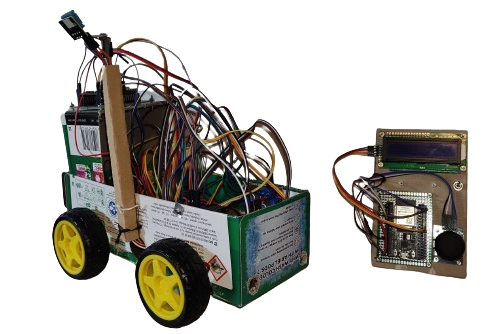
\includegraphics[scale=0.5]{Robot_y_Joystick_1}
   \captionof{figure}{Robot de exploración ambiental.}
   \label{fig:Robot_y_Joystick_1}
\end{center}

El robot de exploración ambiental es un sistema embebido desarrollado sobre \cite{ESP32} utilizando el marco de desarrollo ESP-IDF \cite{ESPIDF_home} de \textit{Espressif Systems} y FreeRTOS (Free Real-Time Operating System) \citep{FreeRTOS} como sistema operativo. Sus principales funciones son la exploración de terrenos de forma controlada por joystick y el la obtención de ciertos parámetros ambientales como luminosidad, presión atmosférica, temperatura y humedad.



\section{Tecnologías backend utilizadas}


\subsection{Amazon Web Services}

AWS (\textit{Amazon Web Services}) \citep{aws}  es una de las principales plataformas de servicios en la nube pública proporcionada por Amazon, que ofrece una amplia gama de productos y herramientas para computación, almacenamiento, bases de datos, redes, inteligencia artificial, seguridad y herramientas de desarrollo.


\subsection{AWS App Runner}

AWS App Runner \citep{aws_app_runner} es un servicio completamente administrado de AWS que permite implementar y ejecutar aplicaciones web y servicios de forma rápida, sin tener que gestionar instancias de infraestructura. Está diseñado para simplificar el proceso de implementación y escalado automático de aplicaciones y permite aplicaciones directamente desde el código fuente o desde contenedores Docker.



\subsection{AWS Glue}

AWS Glue \citep{aws_glue} es un servicio totalmente administrado de AWS diseñado para facilitar la extracción, transformación y carga de datos (ETL) en la nube que permite a los usuarios descubrir, preparar y combinar datos de múltiples fuentes para su análisis y almacenamiento en data lakes, data warehouses o bases de datos. Resulta útil para proyectos de Big Data y análisis de datos ya que brinda un servicio de catálogo de datos, asistencia para la generación de código ETL y un servicio de ejecución de trabajos de procesamiento paralelo.


\subsection{AWS S3}

AWS S3 (\textit{Simple Storage Service}) \citep{aws_s3} es un servicio de almacenamiento de objetos proporcionado por AWS totalmente administrado. Está diseñado para almacenar y recuperar cualquier cantidad de datos desde cualquier lugar, de forma segura, escalable y económica. Es ideal para almacenamiento de datos no estructurado de grandes volúmenes, sitios web estáticos, archivos multimedia, copias de seguridad, etc.

\subsection{AWS Athena}

AWS Athena \citep{aws_athena} es un servicio de análisis de datos serverless proporcionado por AWS que permite consultar directamente datos almacenados en Amazon S3 y los esquemas definidos en Glue, utilizando SQL estándar sin necesidad de configurar ni administrar servidores. Es ideal para analizar grandes volúmenes de datos de forma rápida y económica.



\subsection{MQTT}

MQTT (\textit{Message Queuing Telemetry Transport}) \citep{mqtt_spec} es un protocolo de comunicación asincrónico, ligero y orientado a mensajes, diseñado específicamente para dispositivos con recursos limitados y redes de baja ancho de banda. Es ampliamente utilizado en casos de uso IoT para la transmisión de datos en tiempo real entre dispositivos, sensores y aplicaciones. Utiliza un modelo de comunicacion basado en publish/subscribe y una estructura de datos basada en topics a los cuales los componentes clientes se conectan a un servicio broker para publicar o recibir notificaciones. 

\subsection{AWS IoT Core}

AWS IoT Core \citep{aws_iot_core} es un servicio totalmente administrado de AWS que permite conectar dispositivos IoT (Internet of Things) a la nube de manera segura y confiable. Proporciona una infraestructura escalable para recopilar, procesar y analizar datos de dispositivos en tiempo real, así como para interactuar con otros servicios de AWS a los que se redirigen los mensajes recibidos mediante la configuración de reglas. Tiene soporte para varios protocolos de comunicaciones, entre los que se destacan principalmente MQTT, HTTP/S, WebSockets y LoRaWAN.

\subsection{Node.js}

Node.js \citep{nodejs} es un entorno de ejecución de código abierto, construido sobre el motor de JavaScript V8 de Google Chrome. Aunque debido a su diseño puede ser utilizado para desarrollar aplicaciones backend de propósito general que requieran escalabilidad y rendimiento, es utilizado principalmente como servidor web. Para su funcionamiento utiliza un modelo single-thread de event loop con I/O no bloqueante, por lo que gestiona un bucle de eventos encolados y los procesa invocando sus callbacks de forma asincrónica sin realizar bloqueo de entradas y salidas en los puertos de comunicaciones, permitiendo atención de multiples solicitudes y paralelismo de tareas.

\section{Tecnologías Blockchain utilizadas}


\subsection{Ecosistema Ethereum}

Ethereum \citep{ethereum} es una red blockchain pública diseñada para el procesamiento de transacciones de forma descentralizada con almacenamiento distribuido, inmutable y de acceso libre ( \textit{permissionless}). La red se encuentra formada por los nodos de procesamiento, tambien denominados validadores, que tienen como función procesar transacciones y como otras redes blockchain, utiliza una estructura de datos basada en una cadena de bloques, en los cuales se van agrupando las transacciones validadas. 

Ethereum tiene como \textit{token} el Ether cuyo símbolo es ETH y tiene varios usos, pudiendo ser utilizado como criptomoneda de cambio y ahorro entre los usuarios finales de la red, pero también para pagar el gas (costo de ejecución de transacciones y smart contracts) y los fees a los validadores.

El proceso de validación de transacciones y generación de bloques, a partir de la versión 2.0 de Ethereum, utiliza el protocolo PoS (Proof-of-Stake) \citep{PoS} y opera en ranuras de tiempo llamadas slots, con un bloque propuesto aproximadamente cada 12 segundos. 

El primer paso de este proceso es la recolección de transacciones enviadas por los usuarios a la red (por ejemplo, para transferir dinero o ejecutar contratos) y su almacenamiento en un \textit{mempool} temporal. Luego, un validador es seleccionado de forma aleatoria para proponer el siguiente bloque, seleccionando del \textit{mempool} aquellas transacciones con tarifas de gas mas altas para maximizar su recompensa. El validador seleccionado incluye: las transacciones válidas, estado actualizado del sistema, hash del bloque anterior y los datos adicionales como la firma del bloque. Como resultado, este bloque es propuesto al resto de la red, en la que posteriormente, un comité de validadores, seleccionado de forma aleatoria, revisa el bloque verificando que las transacciones sean válidas, el bloque no esté duplicado o malicioso y sea coherente con el estado de la blockchain. Si el bloque es válido, los validadores emiten un voto (attestation) que confirma su aprobación. Si más de 2/3 de los validadores en el comité atestiguan el bloque, se considera finalizado y el bloque es agregado a la cadena de bloques de forma permanente.

El proceso de compensación y penalización de PoS retribuye a los validadores por diferentes acciones, con el fin de mantener la seguridadm, integridad y consenso de la red, aplica una técnica llamada slashing para la penalización por acciones malisiosas o incorrectas durante el procesamiento. El validador que propone el bloque recibe recompensas por bloque y tarifas de gas. Los validadores que votan correctamente para validar bloques también reciben recompensas proporcionales a su participación. Si el validador no presenta comportamiento malicioso o inactividad, no es penalizado. Sin embargo, los validadores pueden perder parte o todo su capital en stak si proponen múltiples bloques en un mismo slot, o votan de manera inconsistente (por ejemplo, intentando atacar la red), o están inactivos durante largos períodos de tiempo.

Antes de la versión 2.0 de Ethereum, se utilizaba otro protocolo de consenso llamado PoW (Proof-of-Work) \citep{PoW}, en el cual los nodos validadores desempeñaban el rol de mineros que competían por la generación del bloque, recompensando al que lo lograba generar y desaprovechando los recursos de cómputo utilizados por los que no lo lograron. El protocolo PoS en la version actual de Ethereum tiene varias ventajas con respecto a PoW consumiendo un 99,9 \% de energía, aumenta la escalabilidad con técnicas de sharding, y reduce las barreras de entrada al no requerir disponer de un hardware costoso para poder participar del proceso de validación.

% *intro a la evm*

Ethereum se diferencia de otras blockchains, como Bitcoin, porque no es solo un libro mayor digital, sino también una plataforma programable en la cual utilizando un SDK se pueden contruir programas denominados \textit{Smart Contracts} que se despliegan y ejecutan en la red. Como se mencionó anteriormente, los Smart Contracts (o contratos inteligentes) son programas informáticos autónomos que se ejecutan en redes blockchain como Ethereum, Solana o Binance Smart Chain. y están diseñados para automatizar, verificar y hacer cumplir acuerdos sin necesidad de intermediarios. Funcionan bajo el principio de si sucede una condición, entonces ejecutar una acción, aunque también pueden ser invocados de forma directa para operaciones de lectura y escritura. Una vez desplegados en la blockchain, no se pueden modificar, y todas las transacciones quedan registradas públicamente. 

El ciclo de vida de los \textit{smart contracts} comienza con su desarrollo utilizando alguno de los lenguajes de programación y SDK disponibles, como por ejemplo Solidity y Truffle. Una vez desarrollado, tras el proceso de compilación se obtiene un ABI \citep{abi} o especificación del contrato en formato JSON que no es enviado a la blockchain, sino que tiene como proposito poder ser utilizado posteriormente para acceder a los atributos y métodos del mismo a la hora de invocarlo. Posteriormente, durante el proceso de despliegue, se genera un binario del contrato que es enviado a la blockchain y tras ser procesado como una transacción mas, queda disponible en la red de manera inmutable. Al estar desplegado y disponible puede ser invocado o ejecutado automaticamente cuando se cumplen ciertas condiciones, generando nuevas transacciónes inmutables procesadas por la red y disponibles para ser consultadas.

Como se mencionó anteriormente, para la invocación a los \textit{smart contracts} se utilizan las dApps como componente de abstracción. Las dApps son aplicaciones que se ejecutan fuera de la blockchain (pudiendo ser por ejemplo un \textit{backend} en Node.js o un \textit{frontend} Javascript) e interactúan con la blockchain a través de ciertas bibliotecas, como por ejemplo, Web3.js \citep{web3}. Para poder acceder a la red, y posteriormente invocar el \textit{smart contract}, la dApp necesita utilizar un endpoint RPC publicado por cualquier nodo de la red y disponer de la especificación ABI del \textit{smart contract} obtenido durante su compilación (y no se disponible en la red).

Ethereum consta de varias redes disponibles para distintos propósitos. La Mainnet \citep{mainnet} es su red principal para usos productivos. Además existen múltiples \textit{testnets}, o redes de prueba, como Sepolia \citep{sepolia} y Holesky \citep{holesky} entre otras, disponibles para ser usadas durante el desarrollo y evaluación de soluciones blockchain en entornos productivos sin necesidad de pagar con fondos reales. Cada red tiene sus propias características y configuración de parámetros como el consenso, gas \textit{fees} y emisión de bloques.


\subsection{Solidity}

Solidity \cite{solidity} es un lenguaje de programación de alto nivel, orientado a contratos inteligentes, específicamente diseñado para funcionar en la Ethereum Virtual Machine (EVM). Fue creado en 2014 por Gavin Wood, Christian Reitwiessner y otros desarrolladores de Ethereum. Su sintaxis es similar a JavaScript, Python y C++, lo que facilita el aprendizaje para desarrolladores familiarizados con esos lenguajes. 


\subsection{Biblioteca Web3.js}

web3.js \citep{web3} es una biblioteca de JavaScript que permite interactuar con la blockchain de Ethereum y otros protocolos compatibles con Ethereum Virtual Machine (EVM). Proporciona una forma sencilla de conectarse a nodos de Ethereum, realizar transacciones y leer datos de contratos inteligentes, directamente desde aplicaciones web o Node.js.


\subsection{Ganache}

Ganache \cite{ganache_website} es una herramienta de desarrollo de Ethereum que permite crear una blockchain local para probar, desarrollar y depurar contratos inteligentes y dApps de forma rápida y segura. Es parte del conjunto de herramientas de Truffle Suite y es ampliamente utilizada por desarrolladores para simular una red Ethereum sin necesidad de usar una red pública como Mainnet o Testnets (Goerli, Sepolia).


\subsection{Truffle}

Truffle \cite{truffle_website} es un framework de desarrollo para Ethereum y otras blockchains compatibles con EVM (Ethereum Virtual Machine). Es parte de Truffle Suite y proporciona herramientas para compilar, desplegar y probar contratos inteligentes, además de facilitar la gestión de proyectos basados en Web3. Truffle automatiza gran parte del proceso de desarrollo de dApps, reduciendo errores y mejorando la eficiencia.

\subsection{Alchemy}

Como se mencionó mas arriba, la dApp, implementada como un servicio Node.js, es la responsable de invocar al Smart Contract desplegado en Ethereum utilizando un endpoint RPC publicado por cualquier nodo de la red. Debido a que los nodos públicos de la red pueden resultar limitados por motivos de seguridad, rendimiento y confiabilidad, resulta una mejor alternativa levantar un nodo EVM administrado o consumir esto como un servicio de un proveedor como Alchemy. Alchemy \cite{alchemy_website} es una plataforma de desarrollo blockchain que proporciona herramientas e infraestructura para crear y gestionar dApps en Ethereum y otras redes compatibles con EVM. Es conocida como el "AWS de Blockchain" debido a que ofrece nodos como servicio y herramientas para facilitar la interacción con la blockchain sin necesidad de que los desarrolladores configuren y mantengan sus propios nodos. En el trabajo actual, se utilizó Alchemy como punto de integración entre la dApp y los Smart Contracts.

\subsection{Etherscan}

Etherscan \cite{etherscan} es un explorador de bloques y plataforma de análisis para la red Ethereum. Permite a los usuarios buscar, verificar y rastrear transacciones, contratos inteligentes, direcciones de billeteras y otros datos en tiempo real. Es una herramienta fundamental para los desarrolladores y usuarios de Web3, ya que ofrece transparencia y acceso abierto a la información almacenada en la blockchain de Ethereum, tanto la Mainnet como las redes de prueba (Sepolia, Holesky, etc).

\subsection{Metamask}

MetaMask \cite{metamask} es una billetera digital y extensión de navegador (también disponible como aplicación móvil) que permite a los usuarios interactuar con blockchains basadas en Ethereum y otros ecosistemas compatibles con Ethereum, como Binance Smart Chain (BSC) y Polygon. Es una herramienta fundamental para interactuar con aplicaciones descentralizadas (dApps), contratos inteligentes y realizar transacciones de criptomonedas directamente desde tu navegador.
En el presente trabajo se utilizó para almacenar los fondos en ETH obtenidos a través de faucets necesarios para pagar el gas de las transacciones.

\section{Tecnologías de desarrollo utilizadas}


%\begin{center}
%\end{center}
%\includegraphics[scale=0.25]{espressif}

% \footnotetext{Imagen tomada de \cite{espressif-website-esp-idf}}

\subsection{Plataforma Docker}

Docker \cite{docker_website} es un proyecto de código abierto que automatiza el despliegue de aplicaciones dentro de contenedores de software, proporcionando una capa adicional de abstracción y automatización de virtualización de aplicaciones en múltiples sistemas operativos. Docker utiliza características de aislamiento de recursos del kernel Linux, tales como cgroups y espacios de nombres (namespaces) para permitir que contenedores livianos independientes se ejecuten en paralelo de manera aislada evitando la sobrecarga de iniciar y mantener máquinas virtuales.

%\includegraphics[scale=0.15]{docker}



\subsection{Plataforma de CI/CD}
Durante el proceso de desarrollo del producto se utilizó CI/CD (\textit{continuous integration / continuous delivery}) mediante la integración de las siguientes herramientas:

\begin{itemize}
	\item Github \cite{SoftwareTool_Github}: servicio de repositorio y control de versiones de código fuente.
	\item AWS CodePipeline \cite{SoftwareTool_codePipeline}: servicio de compilación, empaquetado y ejecución \textit{builds}.
	\item AWS Elastic Container Registry \cite{SoftwareTool_ECR}: servicio de repositorio y control de versiones de imágenes Docker.
\end{itemize}

El objetivo de esta configuración de servicios es permitir que por cada cambio en el código fuente versionado en el controlador de versiones Github, se dispare un proceso de compilación y ejecución de tests unitarios notificando en tiempo real si dicho cambio agrega o no una falla al actual estado del desarrollo. En caso de pasar satisfactoriamente la compilación y ejecución de los tests entonces se genera una nueva imagen Docker con la última versión del codigo compilado y se versiona en Artifact Registry.

\subsection{Visual Studio Code}

Visual Studio Code \cite{vscode_website} es un editor de código fuente desarrollado por Microsoft para Windows, Linux, macOS y Web. Incluye soporte para la depuración, control integrado de Git, resaltado de sintaxis, finalización inteligente de código, fragmentos y refactorización de código.

%\includegraphics[scale=0.15]{vscode}

\subsection{Sistema operativo Ubuntu}
Ubuntu \cite{ubuntu_website} es una distribución Linux basada en Debian GNU/Linux y patrocinado por Canonical, que incluye principalmente software libre y de código abierto. Puede utilizarse en ordenadores y servidores, está orientado al usuario promedio, con un fuerte enfoque en la facilidad de uso y en mejorar la experiencia del usuario.

%\includegraphics[scale=0.25]{ubuntu}




\chapter{Diseño e implementación} % Main chapter title

\label{Chapter3} % Change X to a consecutive number; for referencing this chapter elsewhere, use \ref{ChapterX}

En este capítulo se presentan los detalles técnicos de diseño e implementación de la solución IoT que se tuvieron en cuenta durante el desarrollo del trabajo.


\section{Arquitectura de software del sistema}


El sistema cuenta con una arquitectura multi-cloud en la que se integra como hardware el robot de exploración ambiental \citep{cese_gonzalo_memoria} desarrollado en el marco de la Carrera de Especialización en Sistemas Embebidos, con un sistema \textit{back-end} desplegado en la nube de Amazon Web Services \citep{aws}, Smart Contracts desplegados en la red Blockchain Ethereum \cite{ethereum}, y un plataforma analítica de datos desplegada en la nube de Azure \cite{azure} utilizando la herramienta Microsoft Fabric \cite{azure_fabric}. 


En la siguiente figura \ref{fig:software_architecture} podemos apreciar la arquitectura de la solución.


\begin{center}
   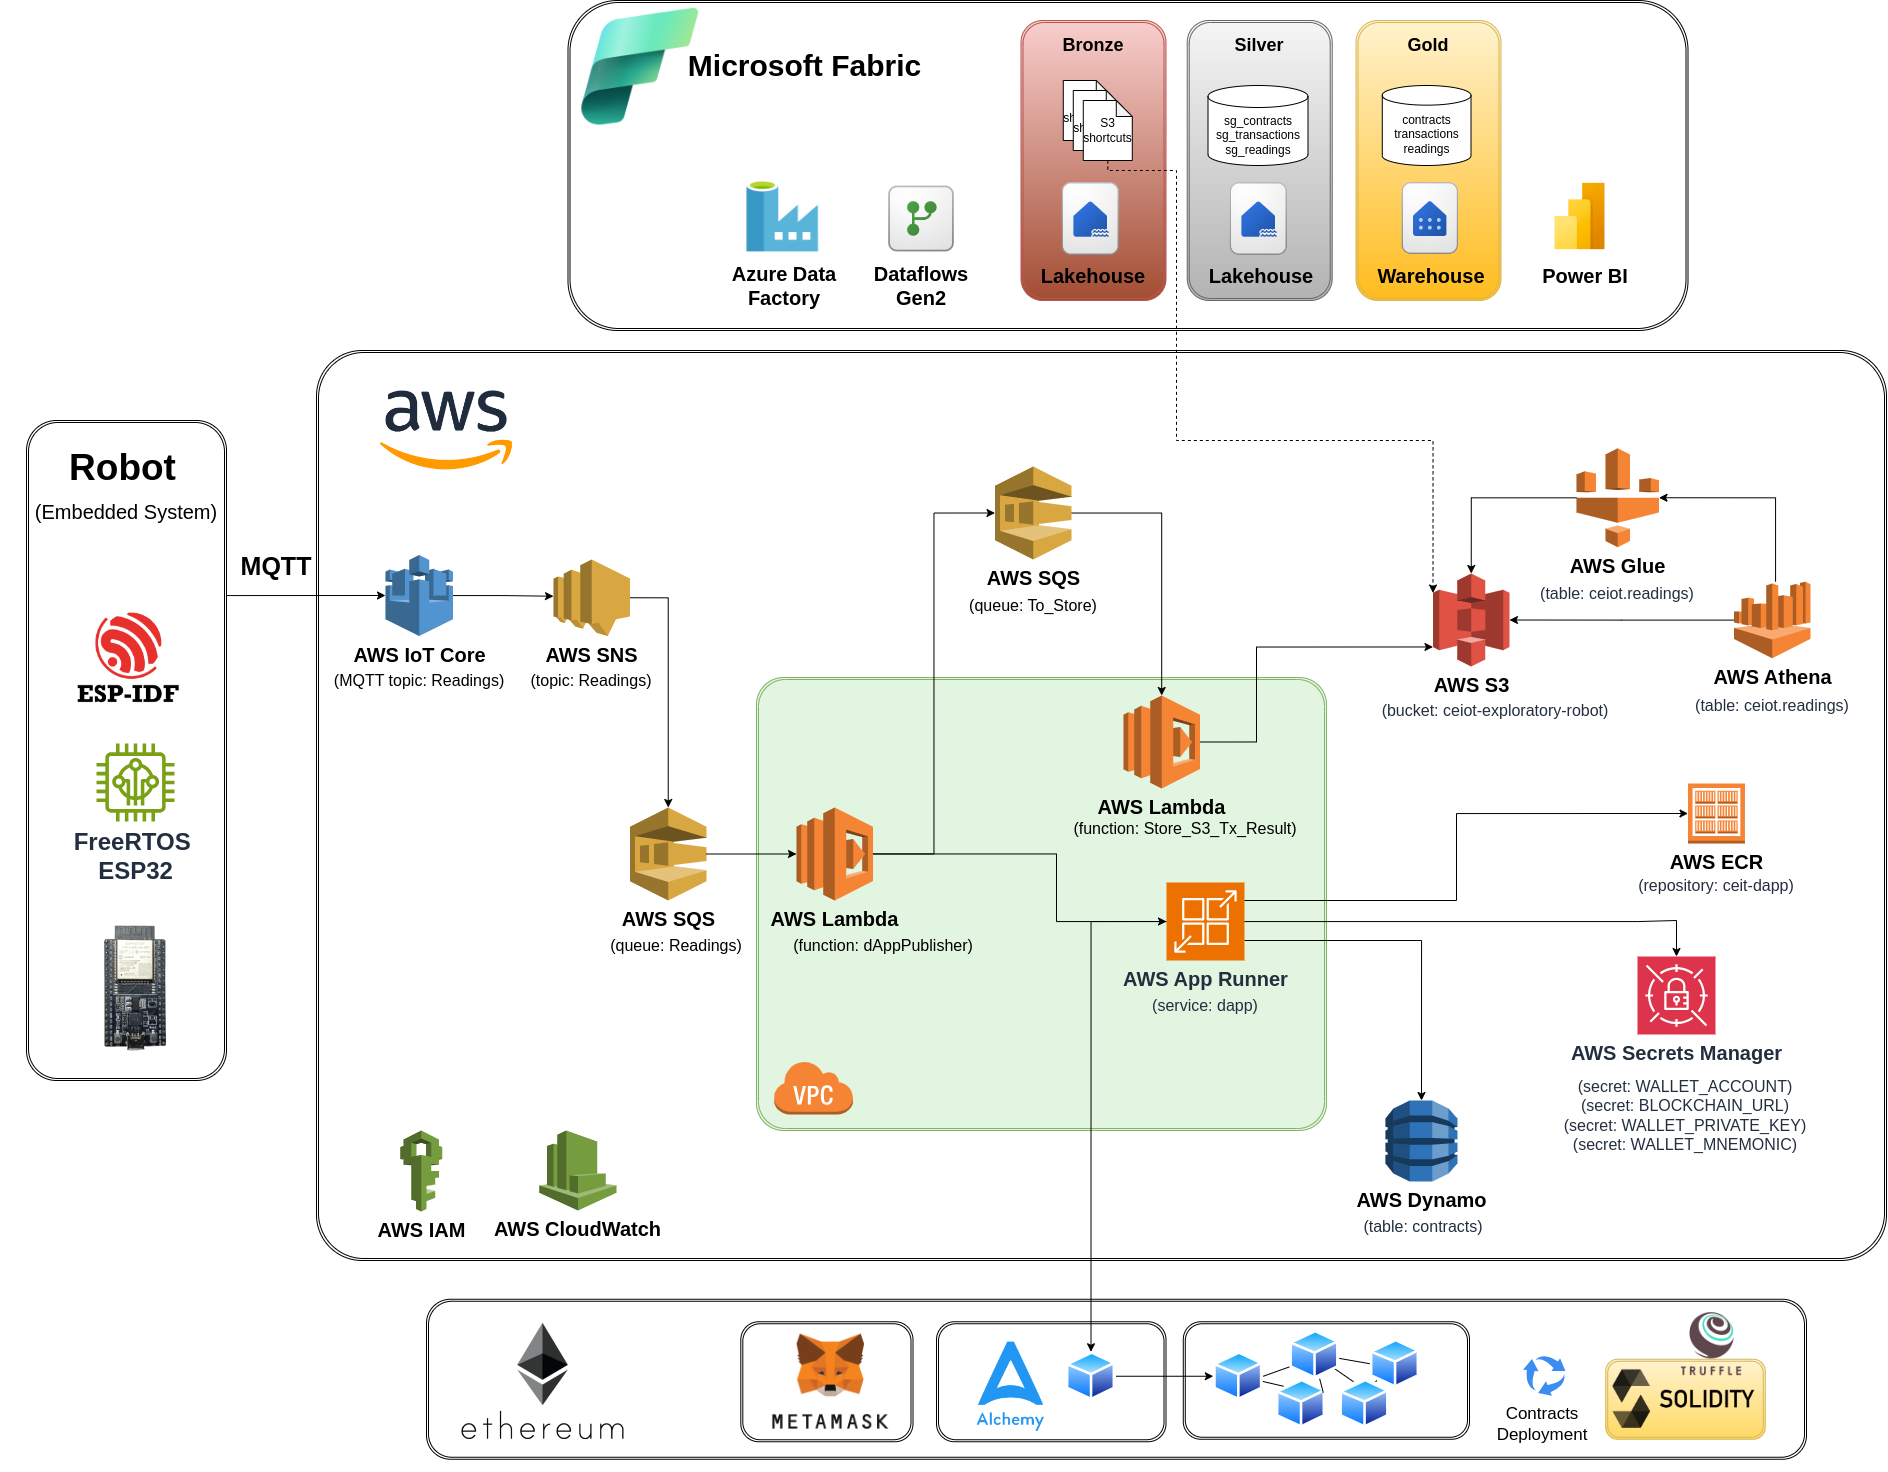
\includegraphics[scale=0.2]{global/software_architecture}
   \captionof{figure}{Arquitectura de la solución.}
   \label{fig:software_architecture}
\end{center}

\section{Hardware e infraestructura del sistema}
 
<A desarrollar>
 
\section{Integración de los módulos y subsistemas}




\subsection{Capa de percepción}


El desarrollo e integración de los componentes de esta capa consistió en la adaptación del firmware desplegado en el robot explorador para extender sus funcionalidades y enviar las lecturas de parámetros ambientales al \textit{topic} MQTT. En la siguiente figura \ref{fig:capa_percepcion} puede apreciarse el conexionado de estos componentes.


\begin{center}
   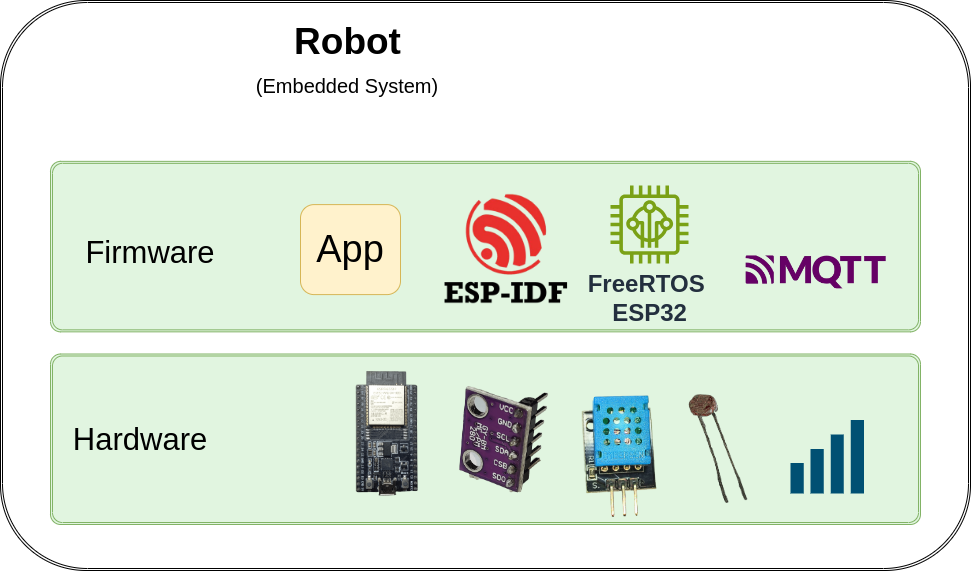
\includegraphics[scale=0.2]{AWS/capa_percepcion}
   \captionof{figure}{Capa de percepción de la solución.}
   \label{fig:capa_percepcion}
\end{center}


Dentro de las funcionalidades que se le agregaron al robot explorador se encontraron:

\begin{itemize}
	\item Capturar fecha y hora local del sistema.
	\item Generación de coordenadas geograficas (con datos \textit{mock}).
	\item Conexión segura con tópico MQTT y envío de los datos generados.	
		
\end{itemize}

La configuración de la fecha y hora se realizó por medio del uso del servicio SNTP \citep{sntp} que permite la sincronización del hardware de una red con la fecha y hora provista por servicios externos en estandar en una zona horaria. Esta configuración se realizó incluyendo el encabezado \textbf{esp\_sntp.h} en el código del robot. Una vez realizado esto fue posible obtener la fecha y hora local invocando a la función \textit{localtime}.

La generación de las coordenadas geograficas con datos \textit{mock} se realizo mediante la generación de las ecuaciones \ref{eq:mock_lat} y \ref{eq:mock_long} a continuación.

\begin{equation}
	\label{eq:mock_lat}
	MockLat = \left( \frac{rand()}{RAND\_MAX} \right) \left( LAT\_MAX - LAT\_MIN \right) + LAT\_MIN
\end{equation}
                
\begin{equation}
	\label{eq:mock_long}
	MockLong = \left( \frac{rand()}{RAND\_MAX} \right) \left( LONG\_MAX - LONG\_MIN \right) + LONG\_MIN
\end{equation}

Finalmente, los datos capturados fueron enviados en formato JSON al tópico MQTT con la estructura de la tabla:


\begin{table}[h]
	\centering
	\caption[caption corto]{Tabla de objetos AWS}
	\begin{tabular}{l c c}    
		\toprule
		\textbf{Nombre del campo} & \textbf{Tipo del campo} & \textbf{Descripción}  \\
		\midrule
		deviceId & string & Id del dispositivo \\		
		type & string & Tipo de lectura \\		
		value & string & Valor de la lectura \\		
		geoLat & string & Latitud geográfica \\		
		geoLong & string & Longitud geográfica\\		
		date & string & Fecha \\		
		time & string & Hora \\		
		
		\bottomrule
		\hline
	\end{tabular}
	\label{tab:json_fields}
\end{table}


A continuación podemos apreciar un valor de ejemplo del objeto JSON enviado por el robot:

\begin{lstlisting}
{   	
	"deviceId": "12ad-dao23-ux23",
	"type": "Temperature",
	"value": "0.00",
	"geoLat": "-26.056772",
	"geoLong": "-64.014824",
	"date": "2025-04-1",
	"time": "11:23:59"
}
\end{lstlisting}

\subsection{Capa de red}

El desarrollo de los componentes de esta capa consistió en la publicación de un \textit{topic} MQTT desde el servicio AWS IoT Core y la configuración de la lógica de redirección y almacenamiento de los mensajes recibidos en AWS S3. En la siguiente figura \ref{fig:capa_red} puede apreciarse el conexionado de los componentes de esta capa.


\begin{center}
   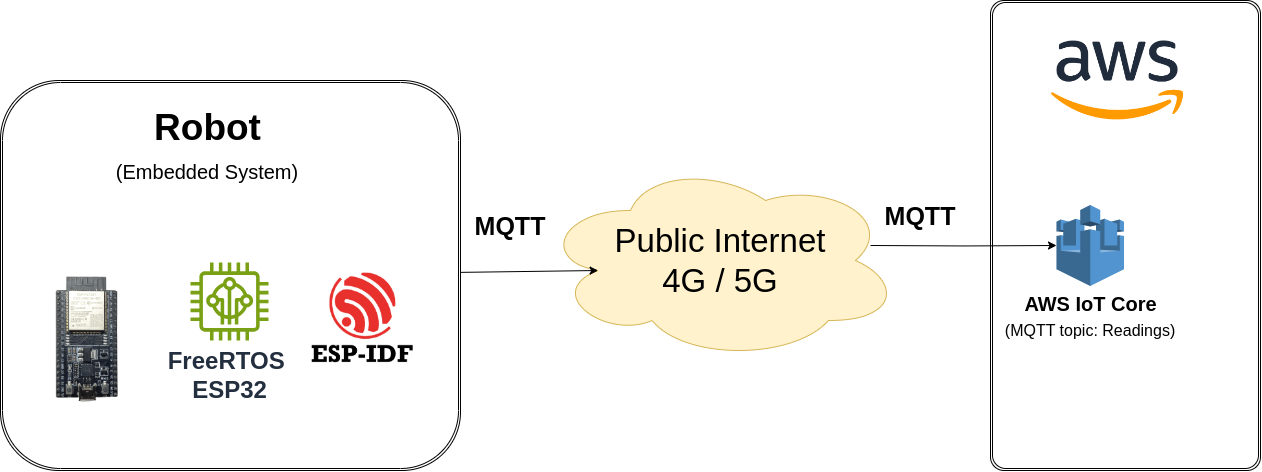
\includegraphics[scale=0.2]{AWS/capa_red}
   \captionof{figure}{Capa de red de la solución.}
   \label{fig:capa_red}
\end{center}

Para la conexión segura con el tópico MQTT se configuró el servicio AWS IoT Core, donde se creó una nueva instancia de un dispositivo remoto con el nombre ESP32. Una vez creado este dispositivo se descargaron e instalaron en el código del robot los certificados listados a continuación:


\begin{itemize}
	\item AmazonRootCA1.pem, renombrado a brokerCA.crt:	Es la autoridad certificadora que AWS usa para firmar certificados de sus servidores. El dispositivo lo necesita para verificar la identidad del servidor AWS IoT al conectarse.
	\item dev-certificate.pem.crt, renombrado a client.crt: Contiene la clave pública correspondiente a la clave privada (.key) y está firmado por AWS (o por una CA en la que AWS confía) para verificar la identidad del dispositivo.
	\item dev-private.pem.key, renombrado a client.key: Usada por el dispositivo para firmar su identidad durante la conexión TLS. Nunca se comparte ni se sube a AWS. Tu dispositivo la usa para autenticar su certificado (.crt).
		
\end{itemize}

Una vez realizada la configuración del servicio AWS IoT core e integrado el robot con el tópico, se probó la recepción de lecturas con el cliente de prueba provisto por AWS suscrito al tópico \textit{readings} como puede apreciarse en la figura \ref{fig:aws_iot_core_mqtt_test_2}.


Para el almacenamiento en AWS S3 de los mensajes recibidos, se configuro una \textit{routing rule} o regla de redirección en AWS IoT Core, indicando mediante una consulta con sintaxis SQL, que todos los mensajes recibidos en el tópico \textit{readings} deben almacernarce en el bucket S3 ceiot-exploratory-robot. En la figura \ref{fig:aws_iot_core_message_routing} puede apreciarse esta configuración.
 


Como resultado de la configuración realizada, los mensajes recibidos en MQTT fueron redirigidos y almacenados en AWS S3 como puede apreciarse en la figura \ref{fig:aws_s3_bucket_data2}.



\subsection{Capas de procesamiento y almacenamiento - dApp (AWS) y Smart Contracts}


El desarrollo de los componentes de esta capa de la solución consta de los elementos de procesamiento que realizan el almacenamiento inmutable de mediciones ambientales en la red Ethereum. En la siguiente figura \ref{fig:capa_blockchain} pueden apreciarse el conexionado de los componentes involucrados.

\begin{center}
   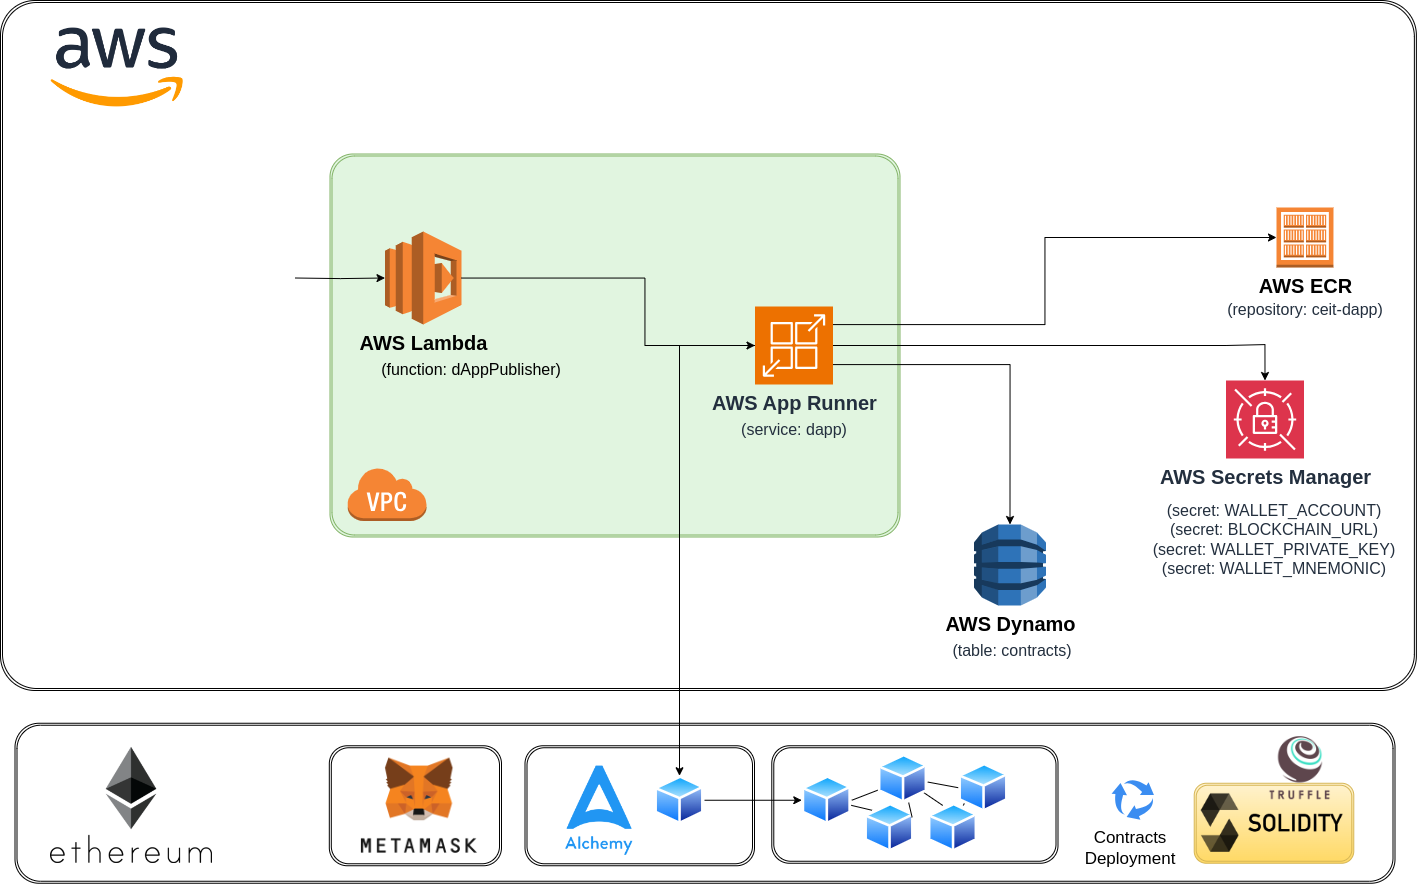
\includegraphics[scale=0.2]{AWS/capa_blockchain}
   \captionof{figure}{Capa blockchain de la solución.}
   \label{fig:capa_blockchain}
\end{center}


Uno de los primeros pasos para poder comenzar a desarrollar los componentes blockchain fue la obtención de tokens para poder realizar despliegues y ejecutar la aplicación en las redes de prueba de Ethereum sin utilizar fondos reales. Para Para poder realizar esto, primero fue necesario crear un \textit{wallet} o billetera digital, para lo que se utilizó el servicio Metamask. Luego, para la obtención de créditos se utilizaron los \textit{faucets} de Google \citep{google_faucets}. Como se puede apreciar en las figura \ref{fig:google_faucets2} y tras seleccionar la dirección del \textit{wallet} y \ref{fig:metamask_balance}, tras realizar las transacciones en el \textit{faucet} se reciben los fondos en la billeta digital. 


Posteriormente como podemos apreciar en la figura, en el servicio Etherscan las transacciones realizadas para generar fondos en la dirección de la billetera quedan publicadas en la red.

Una vez obtenidos los fondos de prueba en la billetera se procedió con el desarrollo de los componentes blockchain. Para el desarrollo de los \textit{smart contracts} se utilizó Solidity como lenguaje de programanción y Truffle como herramienta de gestión de configuración, compilación, empaquetado y despliegue. Truffle utiliza una configuración basada en archivos Javascript para la descripción de las tareas, y para realizar el despliegue a diferentes redes, como por ejemplo de forma local a Ganache o de forma remota a redes como Sepolia, Holesky y Mainnet. En la los archivos de configuración de Truffle se agregaron entradas para poder desplegar a Ganache y a Sepolia como se puede apreciar en la figura \ref{fig:truffle_redes}.

\begin{center}
   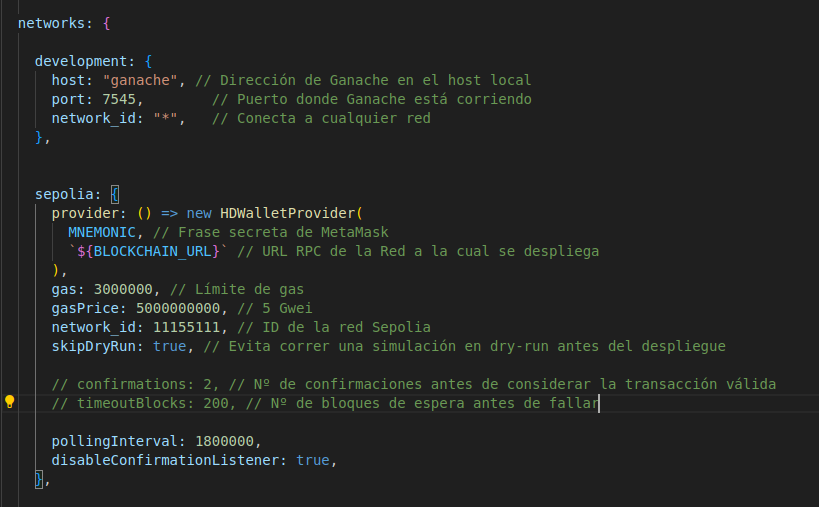
\includegraphics[scale=0.4]{blockchain/truffle_redes}
   \captionof{figure}{Configuración de redes de despliegue en Truffle.}
   \label{fig:truffle_redes}
\end{center}

Como se puede apreciar en la figura \ref{fig:sm_deployment}, durante el proceso de despliegue se presenta cierta información por pantalla:

\begin{itemize}
	\item La red a la cual se esta realizando el despliegue.
	\item Los \textit{smart contracts} incluidos en el despliegue y la dirección que toman una vez desplegados. 
	\item El \textit{hash} o identificador de la transacción.
	\item El número de bloque en el que se encuentra la transacción de despliegue.
	\item La dirección de la billetera digital y el balance disponible previo a la transacción.
	\item La cantidad de gas utilizado en el despliegue, el costo unitario y el costo total de la transacción.
\end{itemize}

Luego de haber realizado el despliegue de los \textit{smart contracts} a la red Sepolia, se puede evidenciar desde Etherscan las transacciones reportadas en la salida por pantalla (figura \ref{fig:sm_deployment_etherscan1}) y comparar los valores. Como se puede apreciar en la figura \ref{fig:sm_deployment_etherscan2}, al ingresar a los detalles de la transacción podemos obtener mas información del contrato.


Desde el punto de vista del \textit{backend} blockchain, se desarrolló la dApp utilizando Node.js y la biblioteca Javascript Web3.js para la comunicación con los \textit{smart contracts}. Para la dApp, se desarrollaron varios \textit{endpoints} y se expusieron mediante el estandar Open API \citep{open_api} utilizando la biblioteca Swagger, que como se puede apreciar en la figura \ref{fig:dapp_endpoints}, genera una interfaz gráfica documenta y brinda un cliente de prueba para poder invocar los \textit{endpoints} expuestos.


Para que la dApp pueda interactuar con la red debe poder conectarse a un endpoint RPC publicado desde cualquier nodo de la misma. Por este motivo se utilizó el servicio Alchemy que brinda publica endpoints para distintas redes, incluyendo Ethereum. Primero se creó un perfil en este servicio de manera gratuita y se creó un nuevo proyecto con el nombre iot\_robots\_storage. Una vez hecho esto se pudo acceder a los diferentes endpoints disponibles de Ethereum para las tres redes principales (Mainnet, Holesky y Sepolia) como se puede apreciar en la figura \ref{fig:alchemy1}. Posteriormente, se configuró en la inicialización de la biblioteca Web3.js en la dApp, el endpoint provisto por Alchemy y el app\_key del proyecto iot\_robots\_storage. 

La dApp fue desplegada utilizando el servicio AWS App Runner por medio de la creación y publicación en AWS ECR de una imagen Docker con el código de la misma. Se configuró el despliegue de la dApp para que se encuentre en una VPC (red privada) con reglas que impiden el tráfico HTTP de ingreso desde la red pública, pero permiten el tráfico saliente, de esta manera la dApp puede acceder al servicio Alchemy e invocar los \textit{Smart Contracts}.

Además de la URL y el key del proyecto en Alchemy, la dApp necesita ciertos datos sensibles para poder acceder a Ethereum, firmar transacciones, y realizar escrituras (ya que dichas operaciones requieren el pago de un fee). Estos datos al ser considerados sensibles, fueron almacenados en el servicio AWS Secret Manager, y accedidos a través del uso de su integración en los diferentes componentes. En la siguiente lista se pueden apreciar el propósito de los mismos:

\begin{itemize}
	\item Wallet Account: identificador unívoco de una cuenta en la red de blockchain.
	\item Wallet Mnemonic: conjunto de entre 12 y 24 palabras que forman la semilla criptográfica para acceder (o recuperar la cuenta) y generar claves privadas, entre otras cosas.
	\item Wallet Private Key: Es generado mediante el Mnemonic, y es necesario para firmar transacciones de escritura.
\end{itemize}


\subsection{Capas de distribución de eventos}

El desarrollo de los componentes de esta capa consta de los elementos de distribución de eventos en tiempo real para permitir el posterior procesamiento y almacenamiento de lecturas ambientales. En la siguiente figura \ref{fig:capa_eventos} puede apreciarse el conexionado de estos componentes.


\begin{center}
   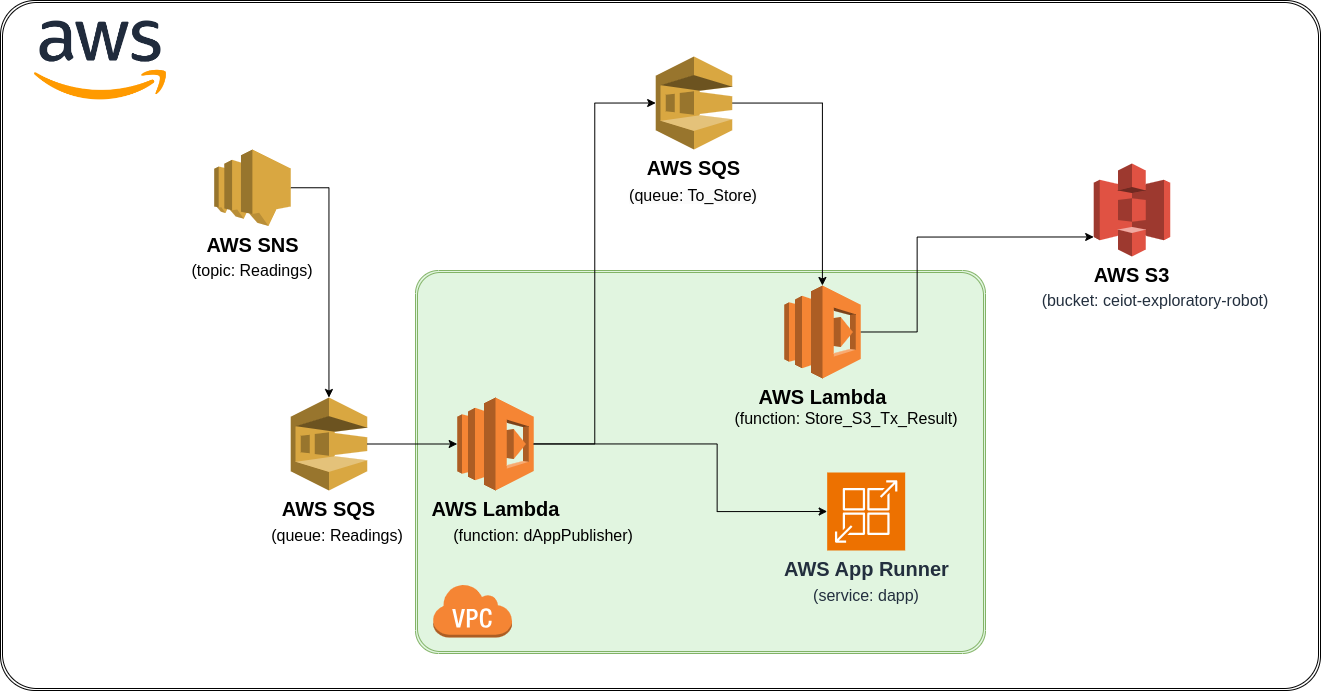
\includegraphics[scale=0.2]{AWS/capa_eventos}
   \captionof{figure}{Capa de eventos de la solución.}
   \label{fig:capa_eventos}
\end{center}


Una vez configurados servicios AWS IoT Core y AWS AppRunner se procedió al despliegue de los componentes que permiten la distribución asíncrona de eventos desde el flujo de ingesta en tiempo real MQTT al posterior almacenamiento en blockchain de las lecturas y en S3 de los resultados de dichas transacciones. Para esto se configuraron los servicios AWS SNS y SQS para brindar, por medio de SNS, una interfaz pub/sub que permita la distribución en paralelo de los eventos recibidos a los topicos suscriptos, y por medio de SQS, un encolamiento de eventos para cada suscriptor de forma que se pueda paralelizar el procesamiento de los eventos.

Dentro de la misma VPC donde se encuentra la dApp (en AWS App Runner) se desplegaron dos funcionas AWS Lambda para la integración entre el flujo de lecturas ambientales, la dApp y el almacenamiento S3:

\begin{itemize}
	\item Send Reading to Blockchain (Python): Implementa la lógica para recibir eventos provenientes de SQS, y construir el request que la dApp espera para poder invocar al Smart Contract pasando los datos como parámetros. Al invocar a la dApp espera la confirmación de la transacción en blockchain y cuando recibe la respuesta la envia a la cola ToStore para ser escrita en S3.
	\item Write Readings and Transactions (Python): Recibe de la cola ToStore la lectura y transacción confirmada, y posteriormente almacena ambos objetos en S3.
\end{itemize}

Desde el punto de vista de infraestructura, como AWS Lambda hace uso de los servicios SQS y S3, que se encuentran expuestos a la red pública, se configuraron AWS Endpoints para integrar la VPC con S3 y SQS de manera interna (sin pasar por la red pública).


\subsection{Capas de procesamiento y almacenamiento de datos}


El desarrollo de los componentes de esta capa consta de los elementos de procesamiento y almacenamiento de los datos para la generación de reportes de negocio. En la siguiente figura \ref{fig:capa_datos} puede apreciarse el conexionado de estos componentes.


\begin{center}
   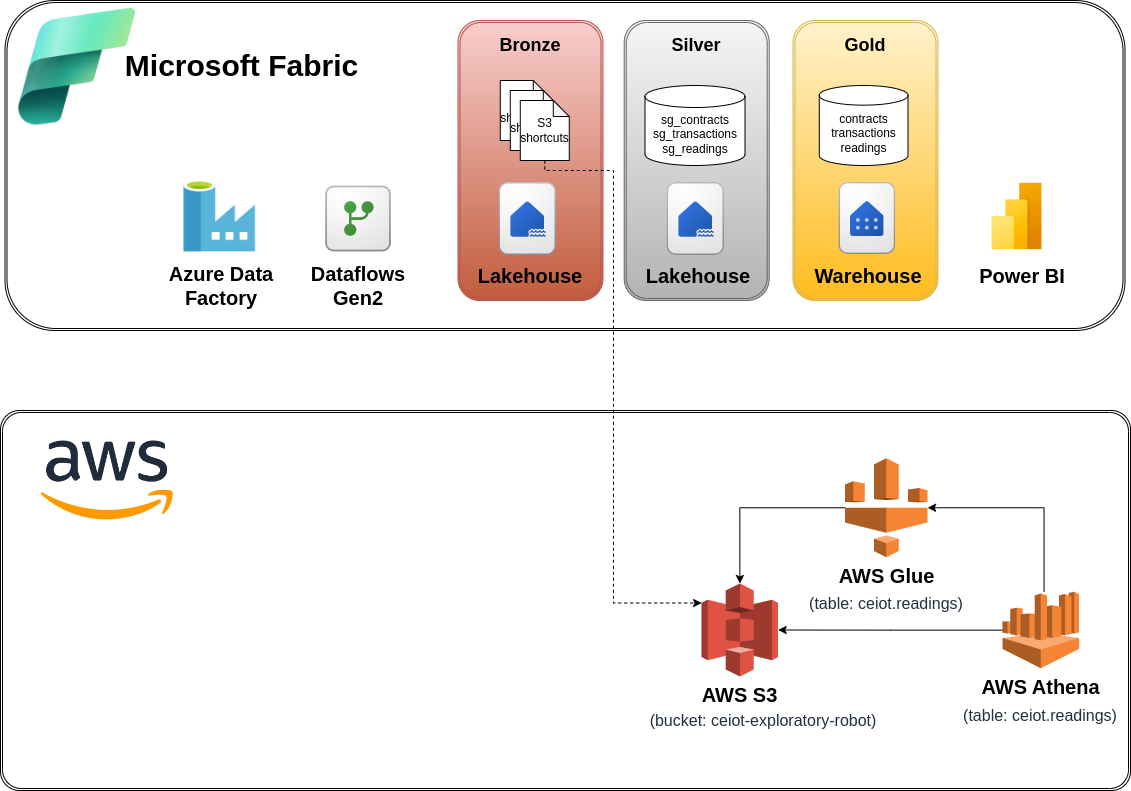
\includegraphics[scale=0.2]{AWS/capa_datos}
   \captionof{figure}{Capa de procesamiento y almacenamiento datos de la solución.}
   \label{fig:capa_datos}
\end{center}

Una vez realizadas las configuraciones de ingesta de datos en \textit{streaming} se realizaron las configuraciones para poder accederlos, administrarlos y procesarlos de forma batch.
Para ello se crearon una base de datos y una tabla en AWS Glue para representar el esquema de datos almacenados en AWS S3 en formato JSON, como se puede apreciar en la figura \ref{fig:aws_glue_table_review}.

%\begin{center}
%   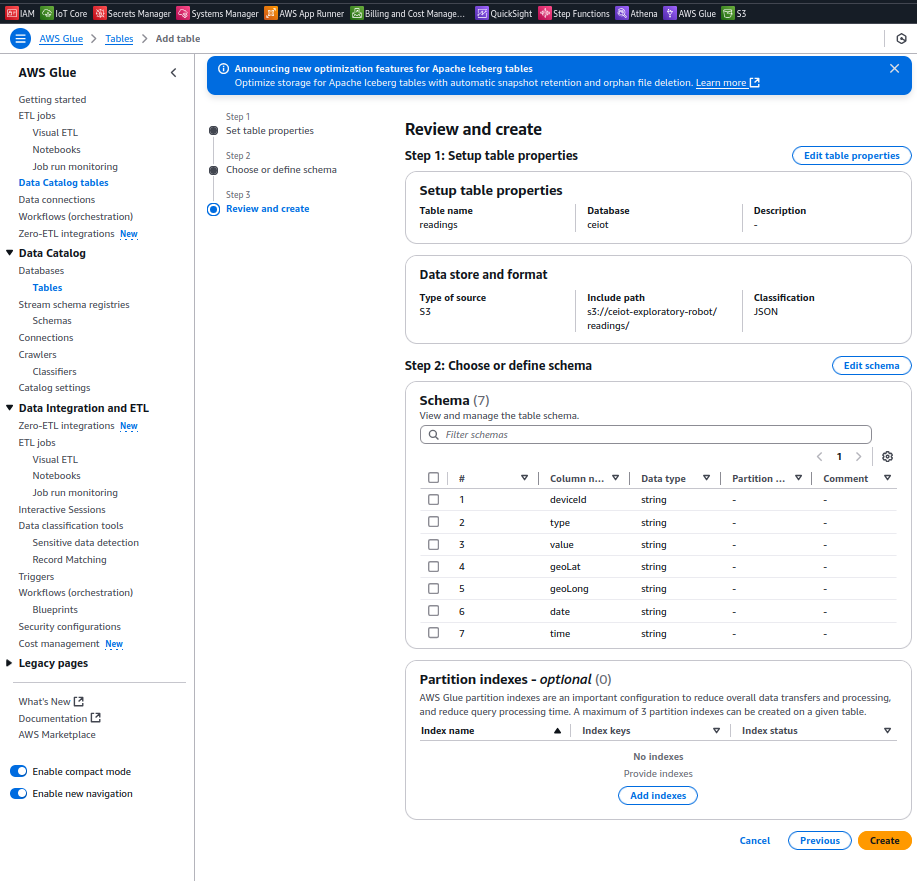
\includegraphics[scale=0.4]{AWS/aws_glue_table_review}
%   \captionof{figure}{Creación de base datos, tabla y esquema AWS Glue.}
%   \label{fig:aws_glue_table_review}
%\end{center}

Con el esquema de datos definido en el catálogo de AWS Glue, fue posible realizar consultas SQL sobre los datos almacenados en AWS S3 desde AWS Athena, como se puede apreciar en la figura 

Para la capa de ingeniería de datos, procesamiento de analíticas y creación de reportes y dashboards, se decidió utilizar la suite de componentes provista por Microsoft Fabric en la nube de Azure.
El diseño de la solución de datos implementada se basó en la arquitectura Medallion donde se implementaron las tres capas estándares (Bronze, Silver y Gold), y se almacenaron los datos en el Data Lake OneLake en formato Delta. La separación en capas se realizó de la siguiente manera:

\begin{itemize}
	\item Capa Bronze: se integró el Fabric Lakehouse con el almacenamiento S3 mediante la configuración de \textit{shortcuts}. Los datos se encontraron almacenados en crudo y con formato JSON.
	\item Capa Silver: se almacenaron y accedieron en el Fabric Lakehouse las tres diferentes entidades (contracts, transactions y readings) en formato de tablas Delta (con archivos Parquet), utilizando el lenguaje SQL a través del SQL Endpoint provisto por Lakehouse. En esta capa los datos se encuentran en estado \textit{staging} en el cual sufren transformaciónes y enrriquecimiento para mejorar su calidad.
	\item Capa Gold: se almacenaron y accedieron el el Fabric Warehouse las tres diferentes entidades (contracts, transactions y readings) como tablas de un modelo relacional SQL. En esta capa los datos se encuentran en su calidad final listos para poder ser entregados y consumidos desde herramientas de visualización y reportes.
\end{itemize}

El proceso de transformación de datos utilizado se baso principalmente en el uso de las herramientas Azure Data Factory y Dataflows Gen2. Con Azure Data Factory se diseñó la orquestación del procesamiento de datos y se utilizaron actividades de copiado y transformación de datos. En la siguiente figura \ref{fig:datafactory_pipeline} puede apreciarse el \textit{data pipeline} en Azure Data Factory:

\begin{center}
   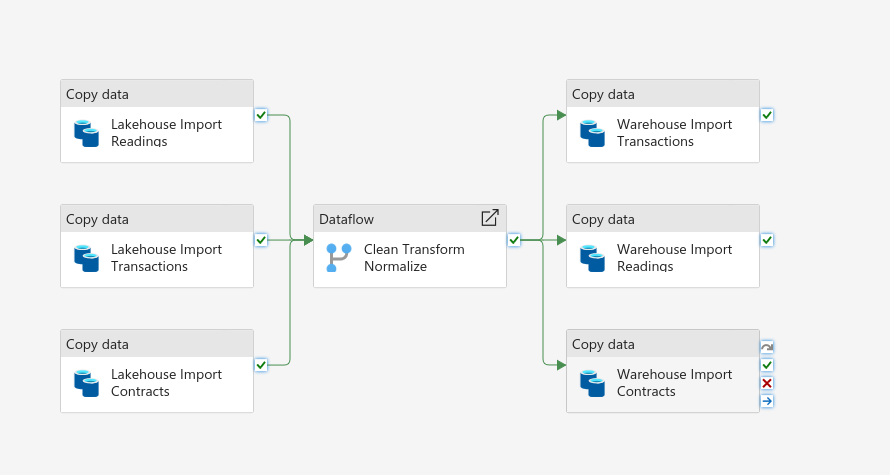
\includegraphics[scale=0.4]{Azure/datafactory_pipeline}
   \captionof{figure}{Azure Data Factory pipeline.}
   \label{fig:datafactory_pipeline}
\end{center}

El flujo esta estructurado de la siguiente manera:
\begin{itemize}

	\item Las tres primeras actividades de movimiento de datos tienen como propósito la copia de datos desde AWS S3 a Fabric OneLake, tranformando el formato de JSON crudo sin compresion a archivos Parquet con compresion Snappy (un 30 por ciento del tamanio original), con la generación y validación del esquema de datos al ser importado como tabla Delta dentro del LakeHouse. Esta actividad se realiza para las tres entidades (contracts, transactions, y readings).
	
	\item La siguiente actividad es la transformación y curado de los datos usando Dataflows Gen2. Los detalles de la misma se explican mas abajo.
	
	\item Finalmente, las ultimas tres actividades son el movimiento de los datos curados en el Lakehouse a la capa Gold en el Warehouse, donde ya se encuentran listos para ser utilizados en el Semantic Model de PowerBI.
\end{itemize}

Para la transformación y limpieza de datos se instanció el componente Dataflows Gen2 desde Azure Data Factory. Posteriormente desde la interfaz de la herramienta Dataflows se configuraron las diferentes actividades de transformación y curado de datos para cada una de las entidades procesadas. En la siguiente figura \ref{fig:dataflows_pipeline} podemos apreciar la orquestasción de estas transformaciones desde Dataflows:

\begin{center}
   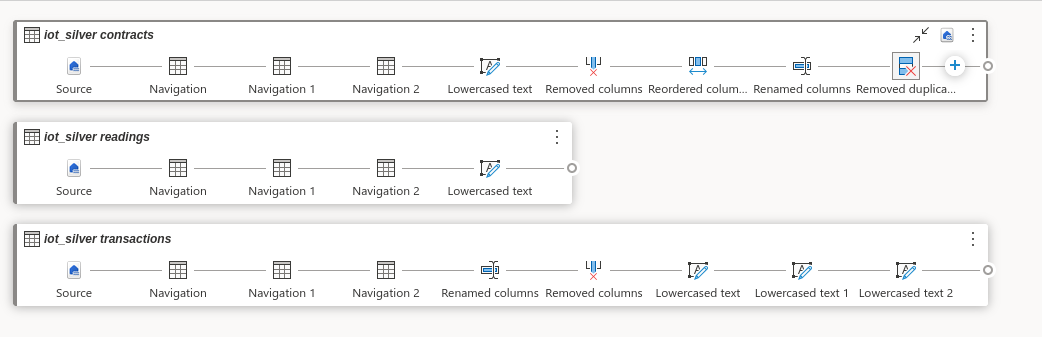
\includegraphics[scale=0.4]{Azure/dataflows_pipeline}
   \captionof{figure}{Dataflows pipeline.}
   \label{fig:dataflows_pipeline}
\end{center}

Como podemos apreciar se aplican diferentes transformaciones dependiendo de la entidad. Las transformaciones realizadas fueron la transformación de los datos a lowercase para algunas columnas con el fin de poder ser cruzadas adecuadamente con las otras entidades, la eliminaación ciertas columnas innecesarias que solo consumen espacio y no resultan de interés para los reportes finales, el reordenamiento de las columnas para la presentación final, y el renombrado  de algunas columnas para estandarizar el acceso.
	
Una vez en el data Warehouse en su capa Gold se creó un Semantic Model de Power BI para poder representar los datos en los reportes. Luego se establecieron las relaciones entre las tres entidades y se crearon ciertas métricas adicionales en para poder facilitar el cálculo dinámico de valores en los dashboards. En la siguiente figura \ref{fig:semantic_model} podemos apreciar una imagen del mismo:

\begin{center}
   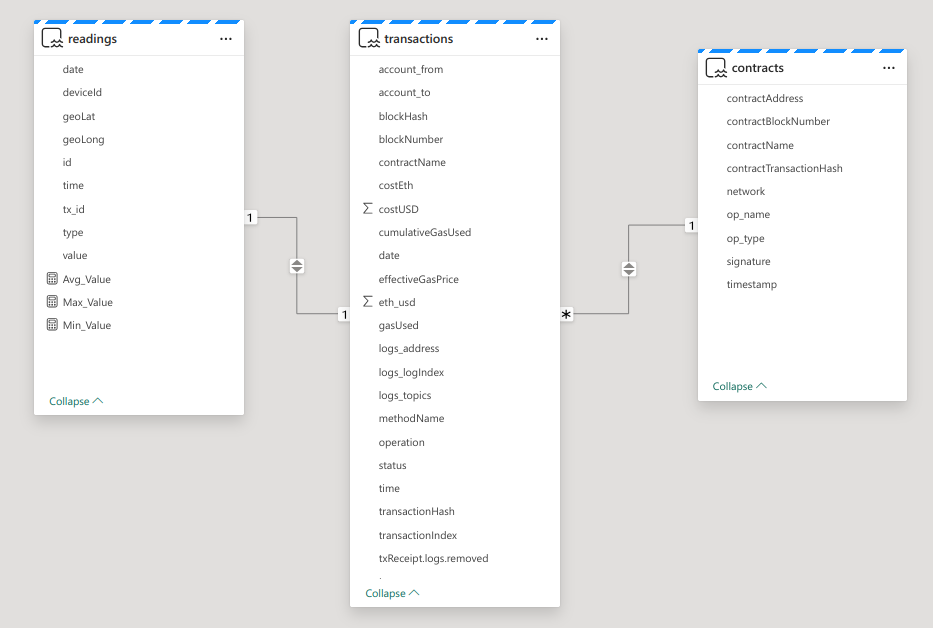
\includegraphics[scale=0.3]{Azure/semantic_model}
   \captionof{figure}{Modelo semántico de PowerBI.}
   \label{fig:semantic_model}
\end{center}

Las métricas creadas fueron:

\begin{itemize}
	\item Readings - Avg Value (valor promedio)
	\item Readings - Max Value (valor máximo)
	\item Readings - Min Value (valor mínimo)
\end{itemize}

Finalmente desde PowerBI se construyeron los reportes compuestos por tablas dinámicas y graficos. Como los datos fueron relacionados en el Semantic Model, al seleccionar valores en el reporte se realiza dinamicamente un filtrado lo cual permite el análisis de la información para la toma de decisiones. En la siguientes figuras \ref{fig:powerbi1} podemos apreciar algunas capturas de algunos de los dashboards generados:



\section{Plataforma de desarrollo y despliegue}



\section{Resumen de todos los objetos cloud creados}


\begin{table}[h]
	\centering
	\caption[caption corto]{Tabla de objetos Azure}
	\begin{tabular}{l c c}    
		\toprule
		\textbf{Servicio} & \textbf{Tipo} & \textbf{Nombre de objeto}  \\
		\midrule
		   ADF & orquestación de actividades & dp-import-and-process \\		
		 Warehouse & almacenamiento estructurado & iot-warehouse \\		
		 Lakehouse & almacenamiento semi-estructurado & iot-lakehouse \\		
		 PowerBI & Reporte & r1 \\	
		 Dataflow & limpieza de datos & df-data-curation \\		
		 Semantic Model & Modelo de datos del reporte & semantic-model \\		
		

		\bottomrule
		\hline
	\end{tabular}
	\label{tab:peces}
\end{table}




\begin{table}[h]
	\centering
	\caption[caption corto]{Tabla de objetos AWS}
	\begin{tabular}{l c c}    
		\toprule
		\textbf{Servicio} & \textbf{Tipo} & \textbf{Nombre de objeto}  \\
		\midrule
		AWS IoT Core & \textit{Thing} & ESP32 \\		
		AWS IoT Core & \textit{MQTT topic} & readings \\		
		AWS IoT Core & \textit{Routing Rule} & StoreToS3 \\		
		AWS S3 & Bucket & ceiot-exploratory-robot \\	
		AWS Glue & \textit Base de datos & ceit \\		
		AWS Glue & Tabla & \textit{readings} \\		
		AWS SNS & \textit Topic & \textit{readings} \\		
		AWS SQS & Queue & \textit{readings} \\	
		AWS SQS & Queue & \textit{toBeStored} \\	
		AWS Lambda & Function & \textit{dAppPublisher} \\	
		AWS Lambda & Function & \textit{StoreS3TxResultsAndReadings } \\	
		AWS App Runner & Service & \textit{dapp } \\	
		AWS Dynamo & Table & \textit{contracts} \\	
		AWS Secrets Manager & Secret & \textit{WALLETACCOUNT} \\	
		AWS Secrets Manager & Secret & \textit{BLOCKCHAINURL} \\	
		AWS Secrets Manager & Secret & \textit{WALLETPRIVATEKEY} \\	
		AWS Secrets Manager & Secret & \textit{WALLETMNEMONIC} \\	
		AWS VPC & VPC & \textit{vpc-b7b022df} \\	
		AWS VPC & Gateway Endpoint & \textit{vpce-075e3abbc2d45ad79} \\	
		AWS VPC & Interface Endpoint & \textit{vpce-0a114cf645105d814} \\	
		AWS VPC & Interface Endpoint & \textit{vpce-0ecc21ebfb9805b08} \\	


		\bottomrule
		\hline
	\end{tabular}
	\label{tab:peces}
\end{table}


% Chapter Template

\chapter{Ensayos y resultados} % Main chapter title

\label{Chapter4} 

En este capítulo se describe el proceso de verificaciones y validaciones que se realizó a fin de comprobar el correcto funcionamiento del sistema y el alcance de los objetivos del trabajo.

%----------------------------------------------------------------------------------------
%	SECTION 1
%----------------------------------------------------------------------------------------

\section{Verificaciones técnicas}



\subsection{Verificación del set-up de dependencias Ethereum}

Como se mencionó anteriormente para poder interactuar con la red Ethereum se necesita disponer de saldo en ETH en un wallet y para esto se utilizaron Faucets de Google. En la siguiente figura \ref{fig:google_faucets2} se puede apreciar la verificación de la obtención de tokens.

\begin{center}
   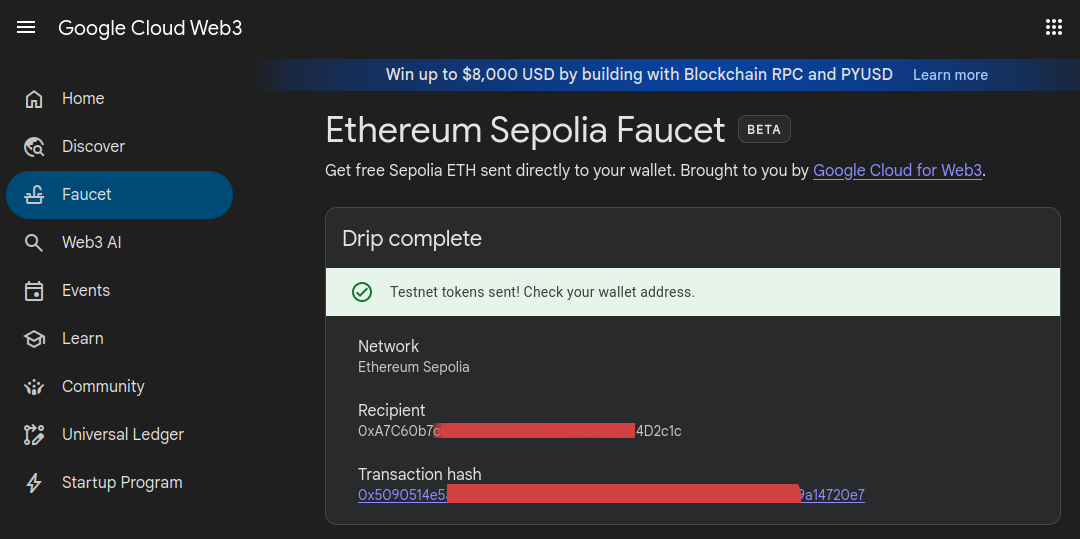
\includegraphics[scale=0.35]{blockchain/google_faucets2}
   \captionof{figure}{Obtención de créditos mediante Google Web3.}
   \label{fig:google_faucets2}
\end{center}

En la figura \ref{fig:metamask_balance} se puede verificar la acreditación de los fondos obtenidos en la billetera Sepolia utilizada para las pruebas. 

\begin{center}
   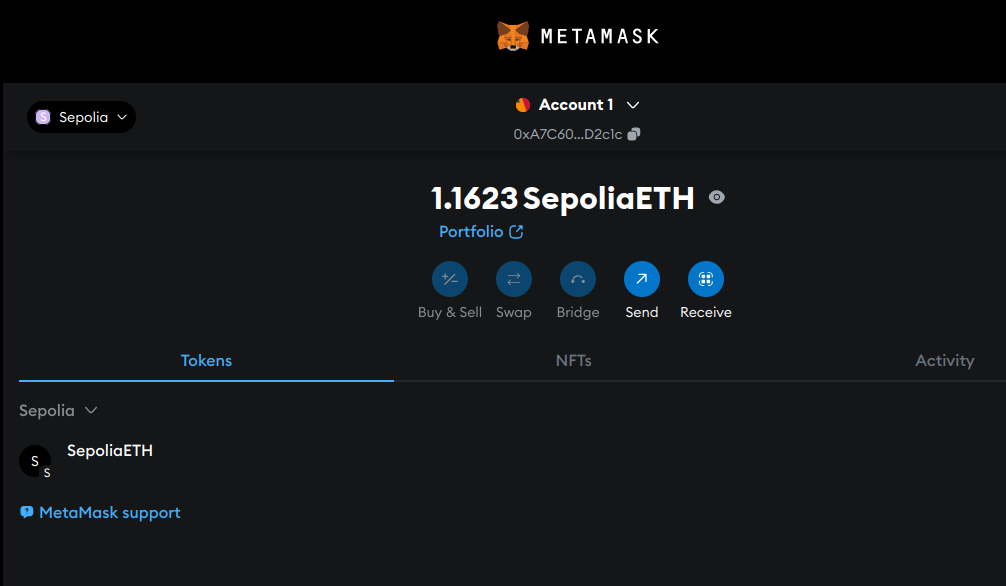
\includegraphics[scale=0.35]{blockchain/metamask_balance}
   \captionof{figure}{Saldo en Metamask.}
   \label{fig:metamask_balance}
\end{center}

Posteriormente se pudo verificar desde Etherscan las transacciones realizadas en la transferencia de los fondos via faucets \ref{fig:sepolia_funding2}.

\begin{center}
   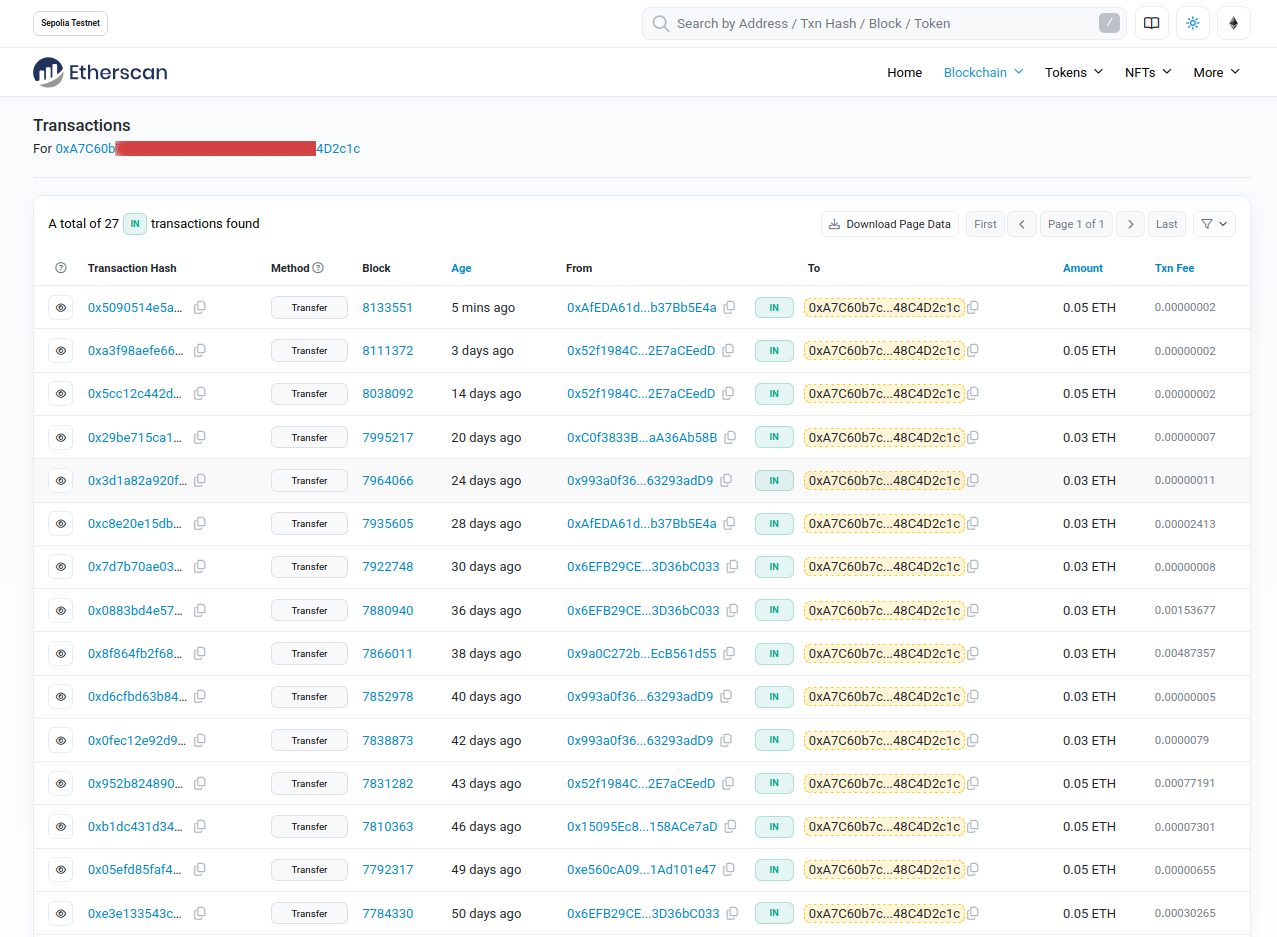
\includegraphics[scale=0.3]{blockchain/sepolia_funding2}
   \captionof{figure}{Transacciones de generación de fondos de prueba.}
   \label{fig:sepolia_funding2}
\end{center}

Como se mencionó anteriormente, el acceso a la red Ethereum se realizó a través del servicio Alchemy. En la siguiente figura \ref{fig:alchemy1} se puede apreciar la verificación de su set-up para poder ser invocado por la dApp. 


\begin{center}
   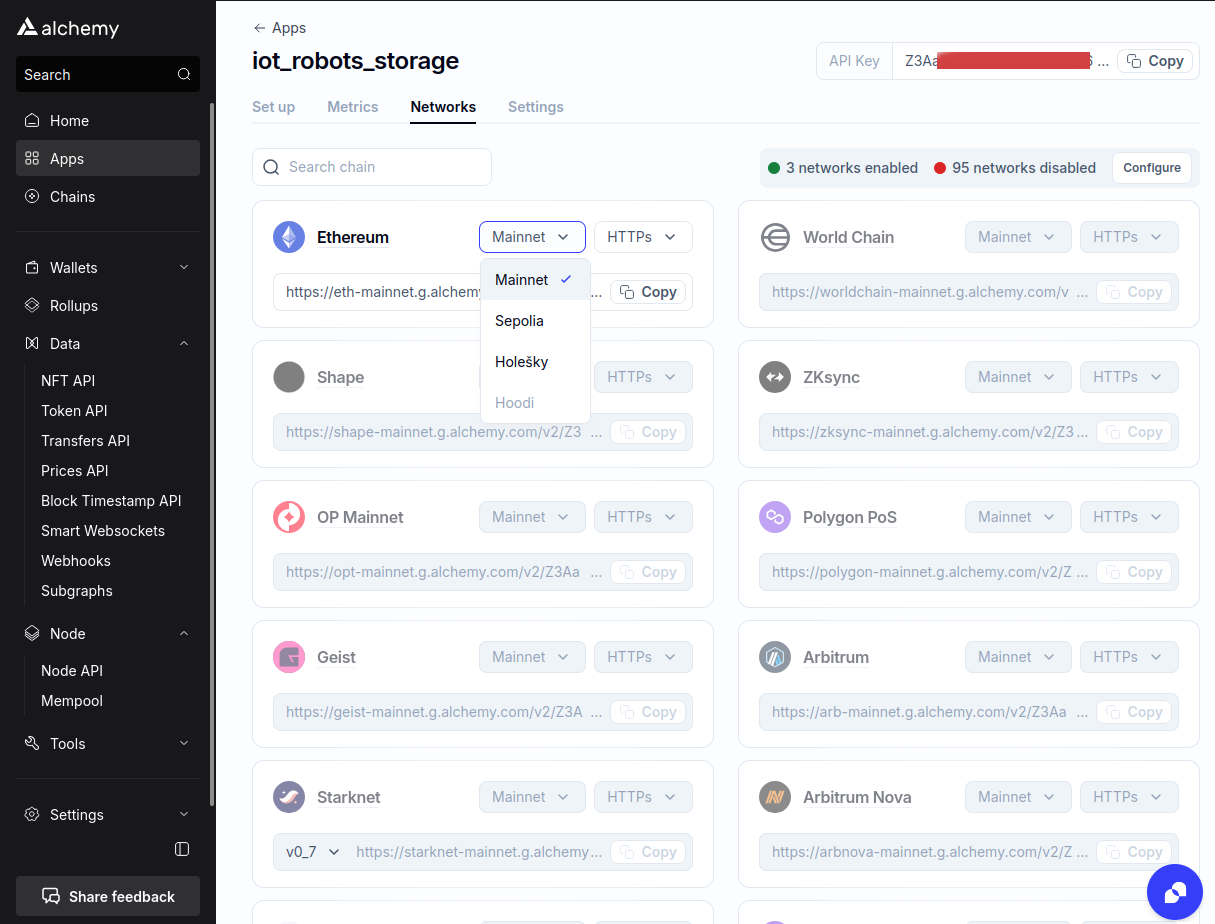
\includegraphics[scale=0.3]{blockchain/alchemy1}
   \captionof{figure}{Frontend the Alchemy.}
   \label{fig:alchemy1}
\end{center}




\subsection{Verificación del despliegue de los Smart Contracts}

Tras ejecutar el proceso de despliegue se pudo verificar la salida por consola con la confirmación del resultado exitoso. Como se puede apreciar en la figura \ref{fig:sm_deployment} se observa la dirección de los Smart Contracts, la cuenta, balance y gas utilizado.


\begin{center}
   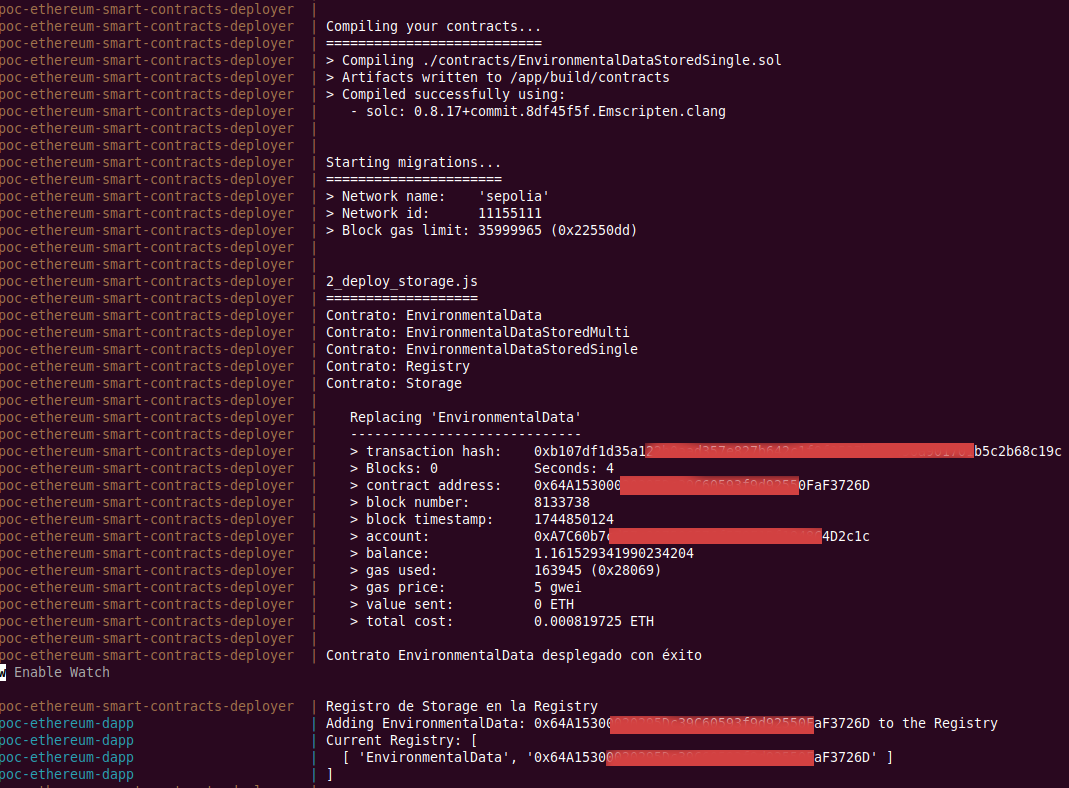
\includegraphics[scale=0.35]{blockchain/sm_deployment}
   \captionof{figure}{Salida por pantalla durante el proceso de despliegue de los componentes blockchain.}
   \label{fig:sm_deployment}
\end{center}

Posteriormente, desde Etherscan se pueden apreciar las transacciones de cada despliegue en la red, por ejemplo en este caso Sepolia, con los detalles de cada una de las operaciones.

\begin{center}
   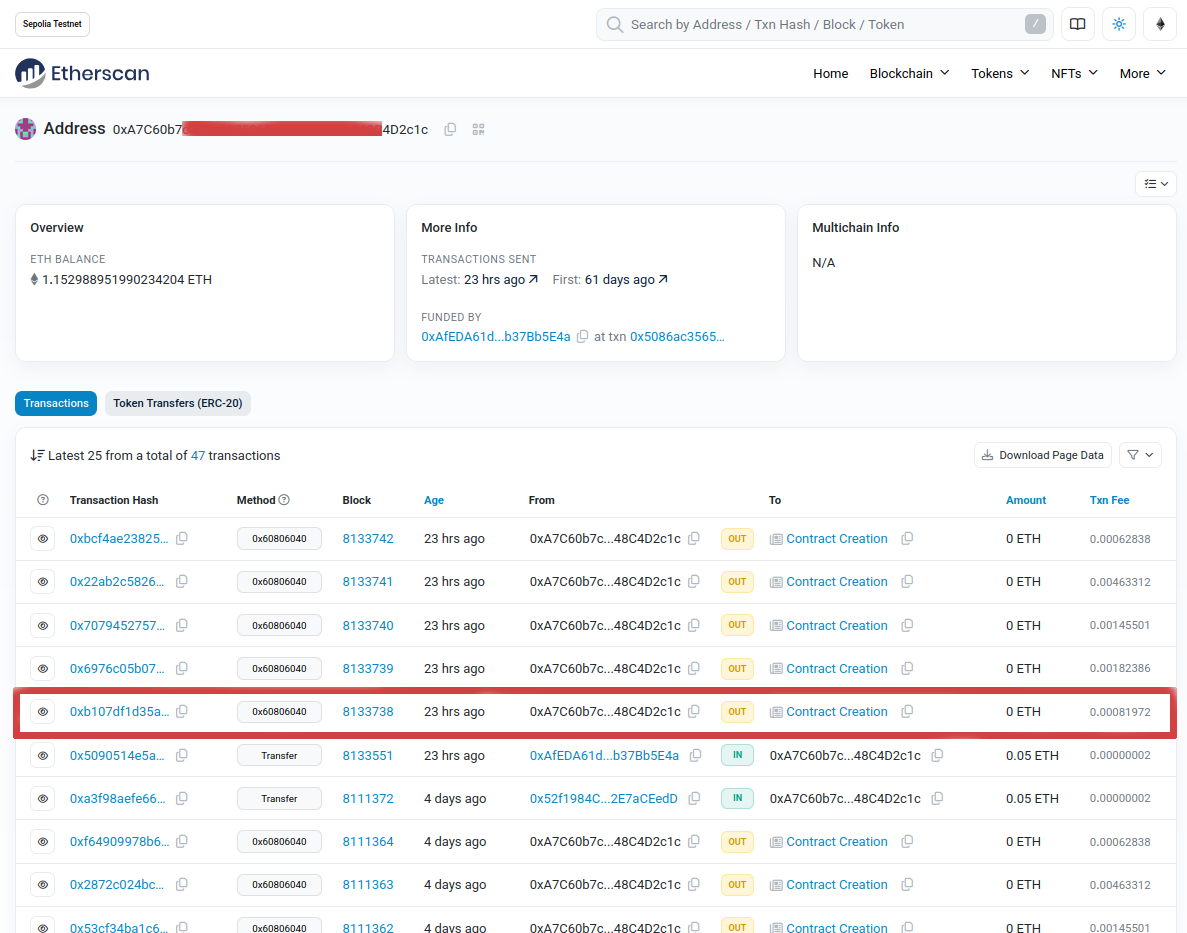
\includegraphics[scale=0.35]{blockchain/sm_deployment_etherscan1}
   \captionof{figure}{Transacciones de despliegue en Sepolia.}
   \label{fig:sm_deployment_etherscan1}
\end{center}

\begin{center}
   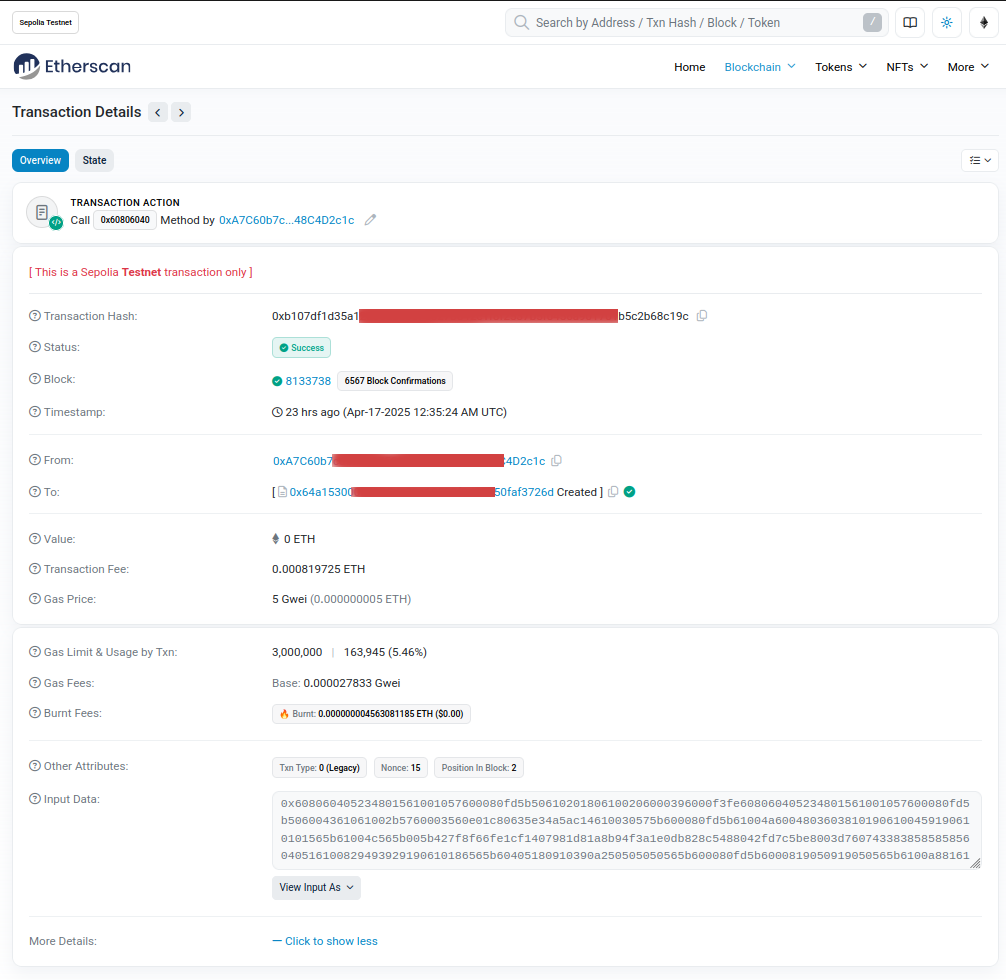
\includegraphics[scale=0.35]{blockchain/sm_deployment_etherscan2}
   \captionof{figure}{Detalles del contrato desplegado en Sepolia.}
   \label{fig:sm_deployment_etherscan2}
\end{center}



\subsection{Verificación del despliegue de la dApp}

Al realizar el despliegue por la consola web de AWS se puede apreciar el resultado exitoso del proceso. Como se observa en la figura \ref{fig:deployment_dapp}, tras el despliegue se puede obtener la URL desde la que se puede acceder a la dapp.

\begin{center}
   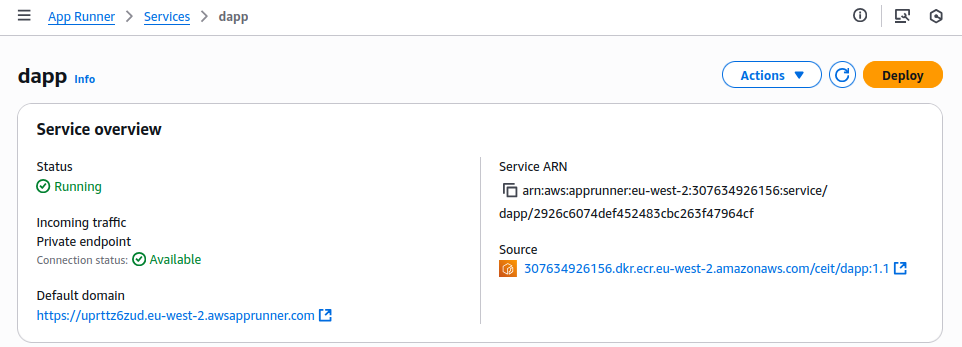
\includegraphics[scale=0.4]{AWS/deployment_dapp}
   \captionof{figure}{Despliegue de la dApp en App Runner.}
   \label{fig:deployment_dapp}
\end{center}

Como se puede apreciar en la siguiente figura \ref{fig:deployment_dapp_log} los logs del despliegue indican que el proceso se realizó exitosamente y se puede apreciar el historial de últimos despliegues.

\begin{center}
   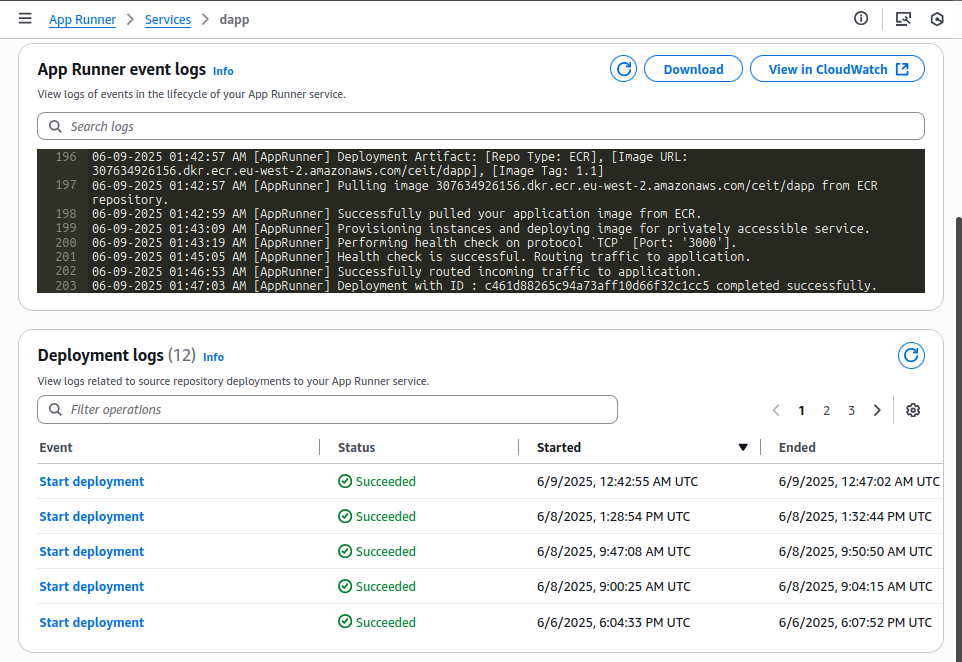
\includegraphics[scale=0.4]{AWS/deployment_dapp_log}
   \captionof{figure}{Despliegue de la dApp en App Runner.}
   \label{fig:deployment_dapp_log}
\end{center}

Una vez verificado el despliegue en la consola de AWS se puede apreciar en la figura \ref{fig:dapp_endpoints} la verificación del funcionamiento de la dApp accediendo a su API Restful publicada por Swagger.


\begin{center}
   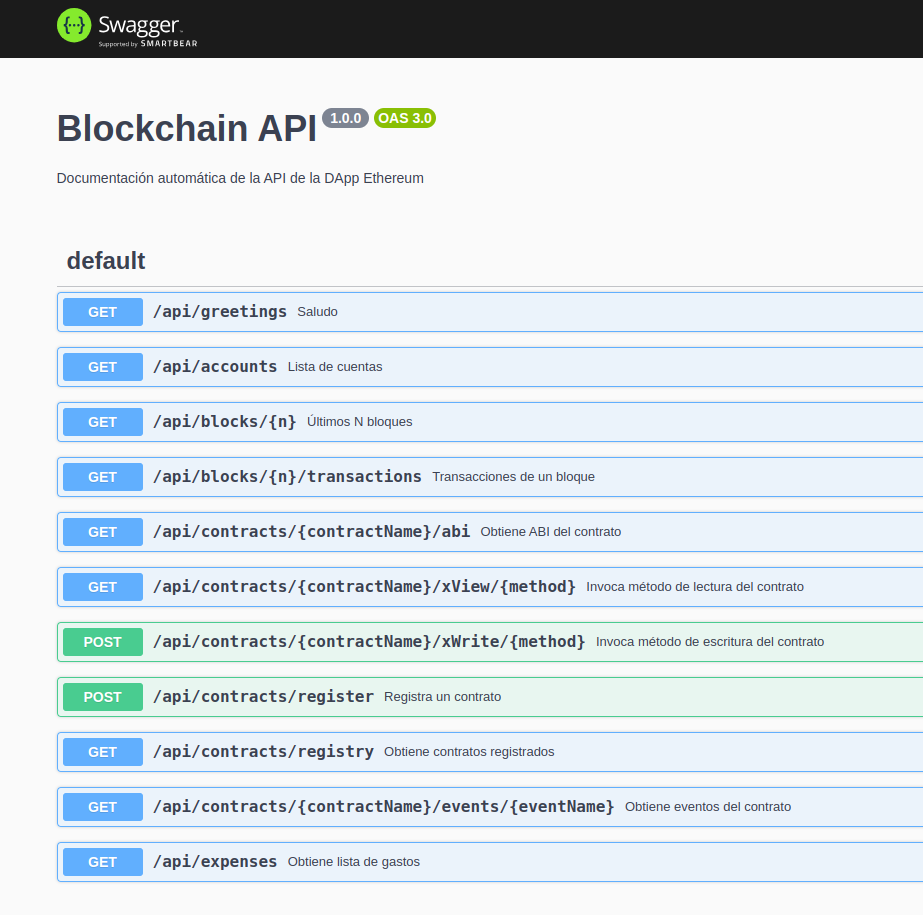
\includegraphics[scale=0.4]{blockchain/dapp_endpoints}
   \captionof{figure}{Endpoints expuestos por la dApp.}
   \label{fig:dapp_endpoints}
\end{center}


\subsection{Verificación de ingesta de datos en tiempo real MQTT}

Desde la herramienta AWS IoT Core se pudo verificar la recepción de mensajes MQTT desde el dispositivo ESP32 como se puede apreciar en la siguiente figura \ref{fig:aws_iot_core_mqtt_test_2}.

\begin{center}
   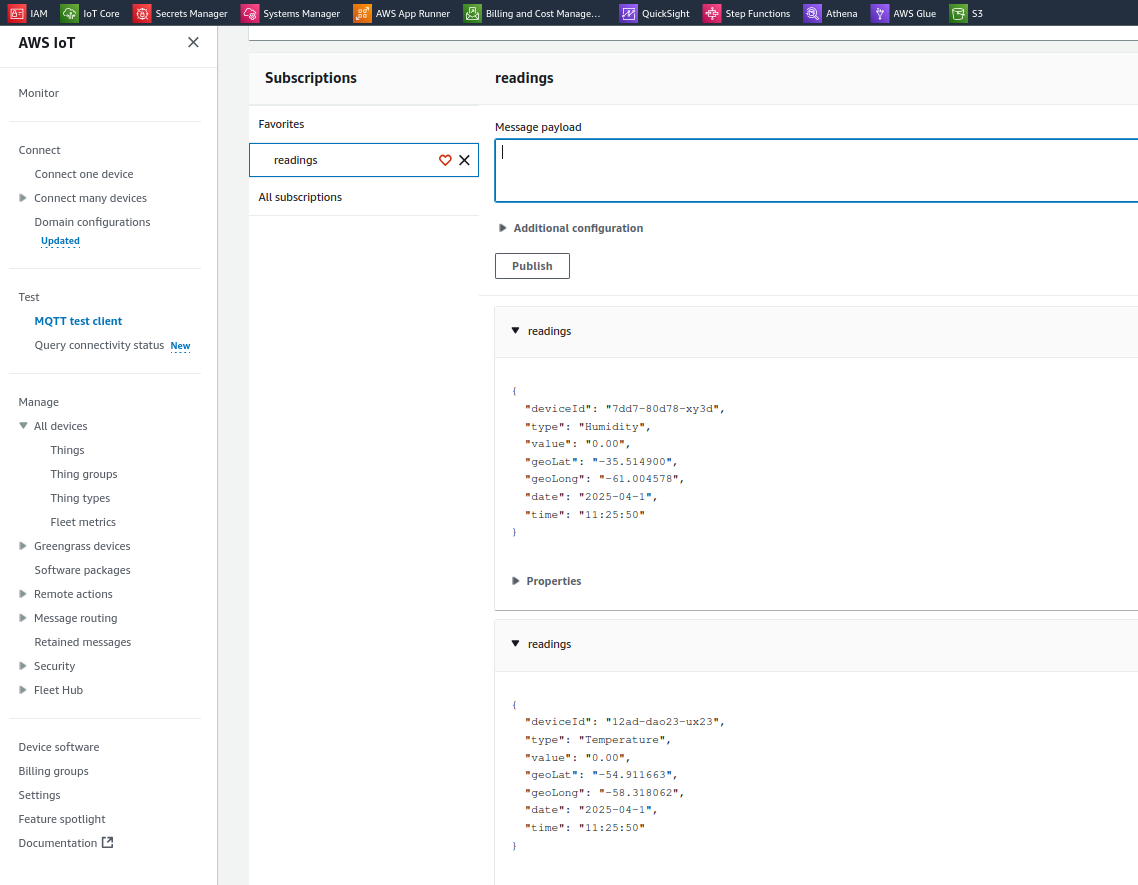
\includegraphics[scale=0.35]{AWS/aws_iot_core_mqtt_test_2}
   \captionof{figure}{Prueba de recepción de mensajes MQTT.}
   \label{fig:aws_iot_core_mqtt_test_2}
\end{center}


\subsection{Verificación del procesamiento de mensajes }

Una vez redireccionados desde AWS IoT Core por medio de AWS SNS, se pudo verificar el encolamiento de los mensajes en AWS SQS donde como se puede apreciar en la figura \ref{fig:events_sqs_2}, los mensajes se acumulan para ser procesados en la cola \textit{readings}.

\begin{center}
   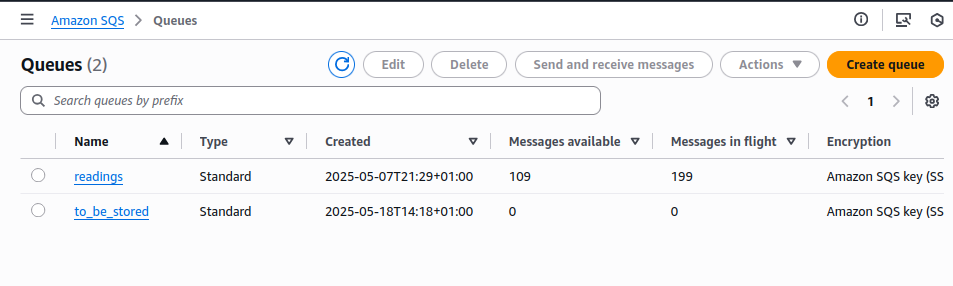
\includegraphics[scale=0.4]{AWS/events_sqs_2}
   \captionof{figure}{Configuración de redirección de mensajes MQTT.}
   \label{fig:events_sqs_2}
\end{center}

Como se aprecia en la siguiente figura \ref{fig:events_sqs_1}, también se pudo verificar la tasa de invocaciones de AWS SQS desde su herramienta de monitoreo.

\begin{center}
   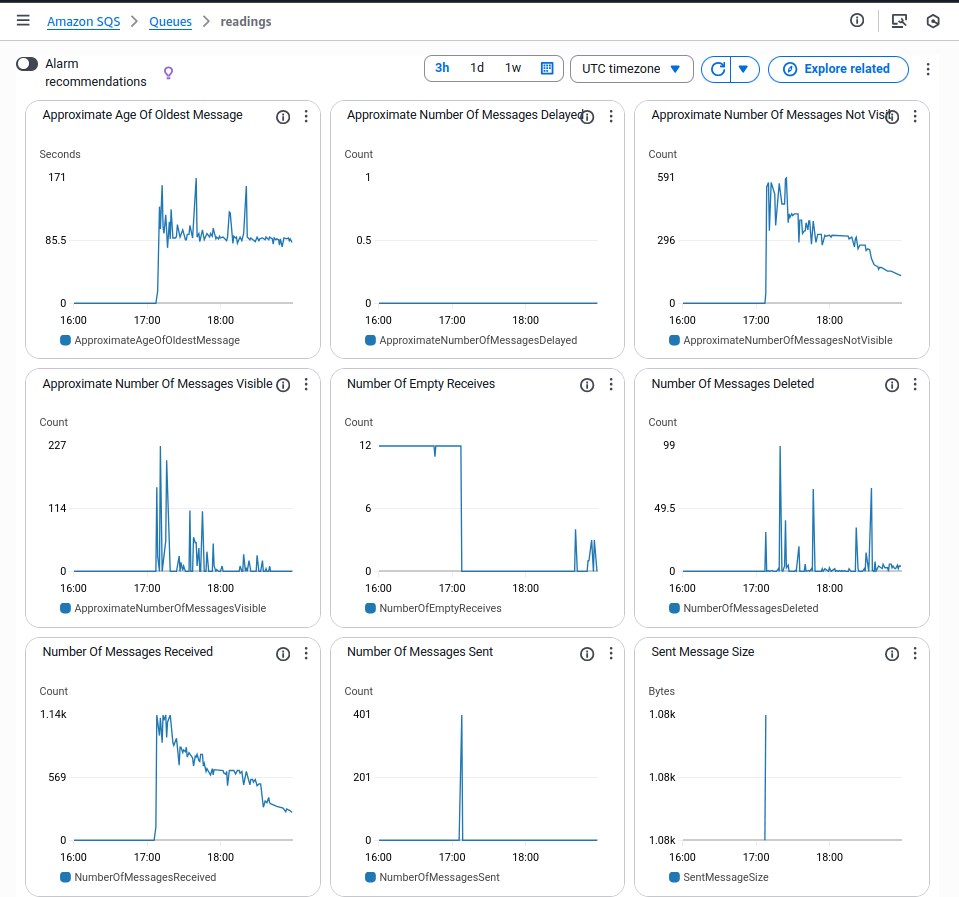
\includegraphics[scale=0.4]{AWS/events_sqs_1}
   \captionof{figure}{Configuración de redirección de mensajes MQTT.}
   \label{fig:events_sqs_1}
\end{center}


Como se mencionó anteriormente, desde la cola readings se dispara la ejecución de la función AWS Lambda que procesa los mensajes, invocando la dApp. Como se puede apreciar en la siguientes figuras \ref{fig:events_lambda1} y \ref{fig:events_lambda3}, se verificó el correcto funcionamiento del procesamiento de eventos.


\begin{center}
   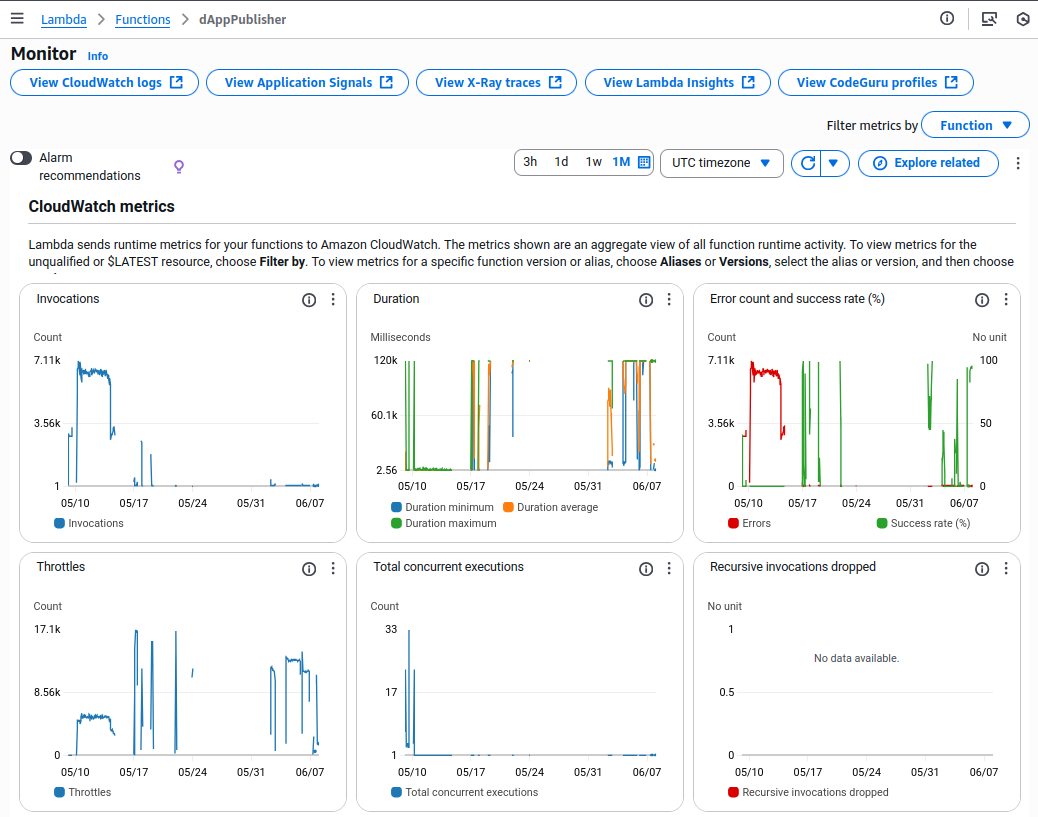
\includegraphics[scale=0.4]{AWS/events_lambda1}
   \captionof{figure}{Monitoreo de la función AWS Lambda de procesamiento de eventos.}
   \label{fig:events_lambda1}
\end{center}

\begin{center}
   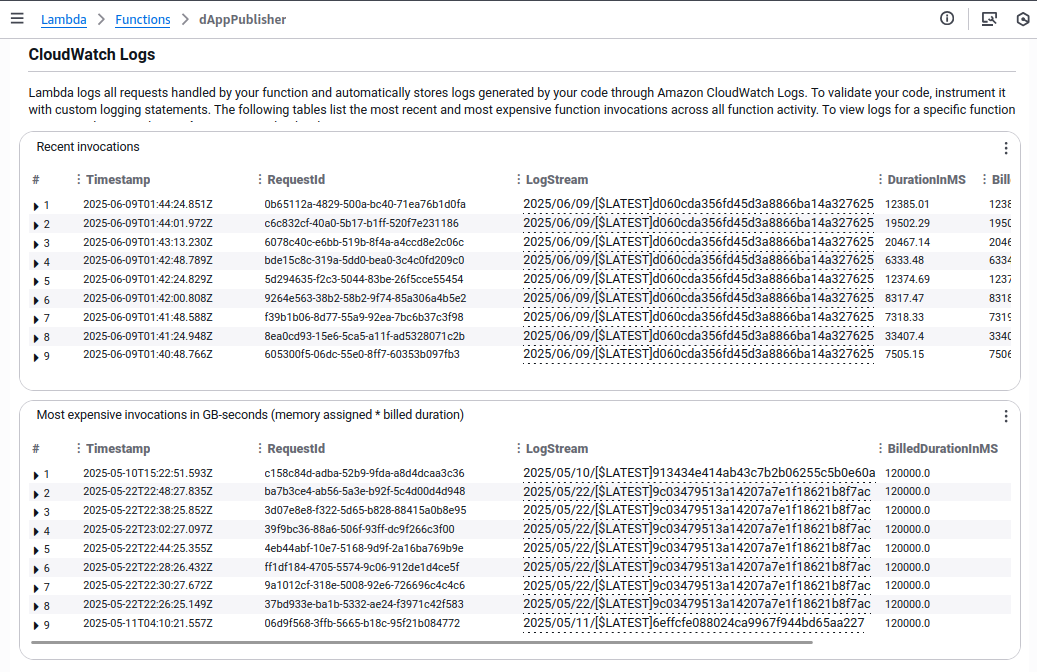
\includegraphics[scale=0.4]{AWS/events_lambda3}
   \captionof{figure}{Monitoreo de la función AWS Lambda de procesamiento de eventos.}
   \label{fig:events_lambda3}
\end{center}

\begin{center}
   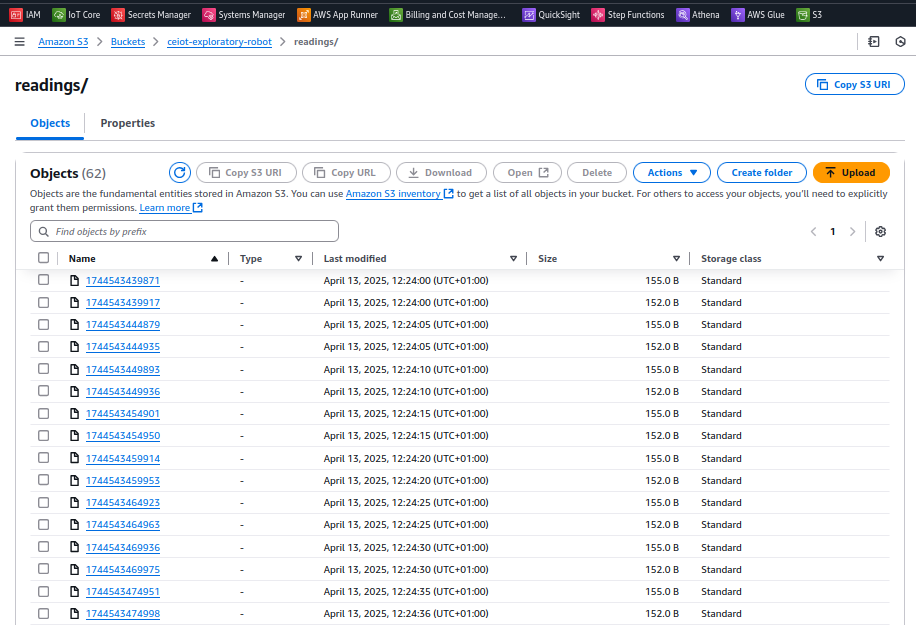
\includegraphics[scale=0.4]{AWS/aws_s3_bucket_data2}
   \captionof{figure}{Almacenamiento de mensajes JSON en AWS S3.}
   \label{fig:aws_s3_bucket_data2}
\end{center}



\subsection{Verificación de la invocación de la dApp y los Smart Contracts}

En la dApp, se pudo verificar el correcto funcionamiento del sistema en sus herramientas de monitoreo como se puede apreciar en las siguientes figuras \ref{fig:events_dapp} y \ref{fig:events_cloudwatch_dapp} las métricas de request HTTP y los logs de las transacciones Ethereum.


\begin{center}
   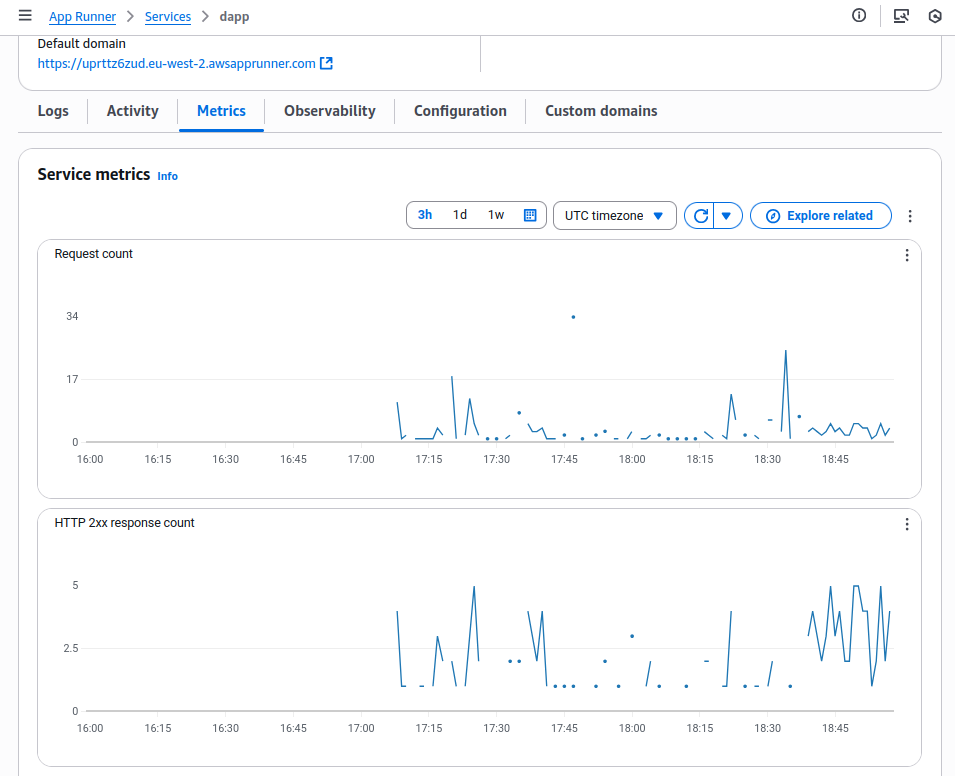
\includegraphics[scale=0.4]{AWS/events_dapp}
   \captionof{figure}{Almacenamiento de mensajes JSON en AWS S3.}
   \label{fig:events_dapp}
\end{center}

\begin{center}
   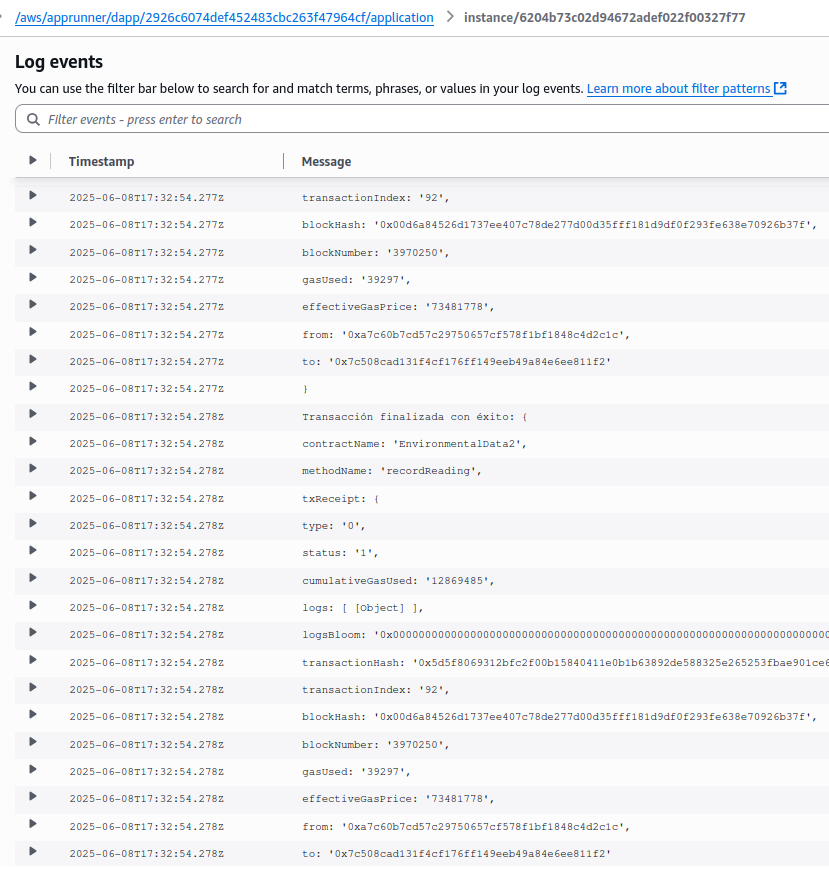
\includegraphics[scale=0.4]{AWS/events_cloudwatch_dapp}
   \captionof{figure}{Logs en Cloudwatch de las transacciones.}
   \label{fig:events_cloudwatch_dapp}
\end{center}


\subsection{Validación de los datos almacenados en Ethereum}


Por cada ejecución tambien se pudo verificar en Etherscan la creación de nuevas transacciones tras la ejecución de la dApp, como se puede apreciar en la figura \ref{fig:events_etherscan}.

\begin{center}
   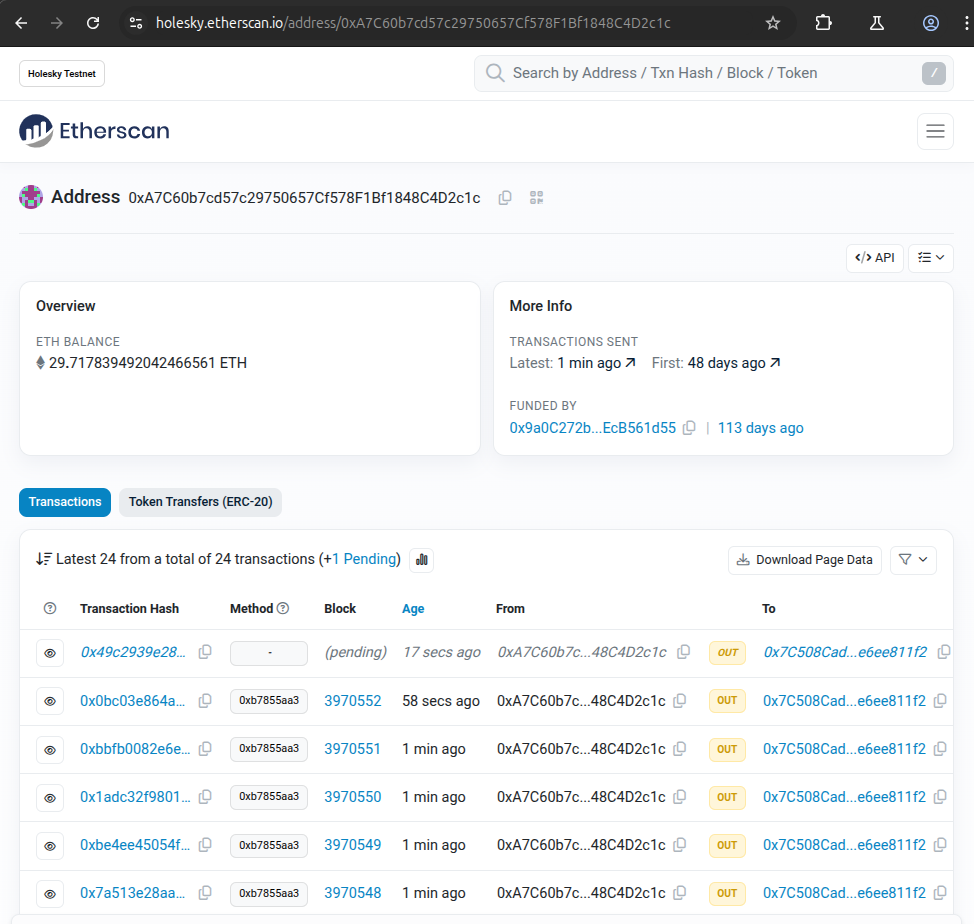
\includegraphics[scale=0.4]{AWS/events_etherscan}
   \captionof{figure}{Creación de nuevas transacciones en Etherscan.}
   \label{fig:events_etherscan}
\end{center}


\subsection{Verificación del proceso de almacenamiento de lecturas, transacciones y contratos en AWS S3}

Como se puede apreciar en las figuras se pudo verificar en AWS S3 el correcto almacenamiento de los objetos datos de lecturas, transacciones y contratos en el bucket configurado.

\begin{center}
   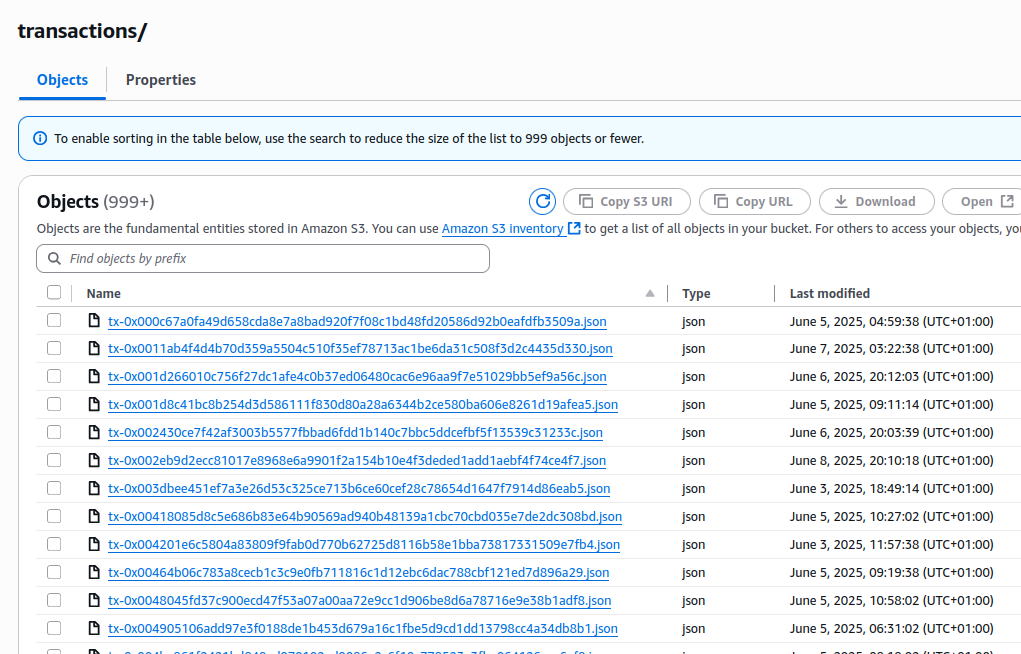
\includegraphics[scale=0.4]{AWS/events_s3_tx}
   \captionof{figure}{Almacenamiento de mensajes JSON en AWS S3.}
   \label{fig:events_s3_tx}
\end{center}


\begin{center}
   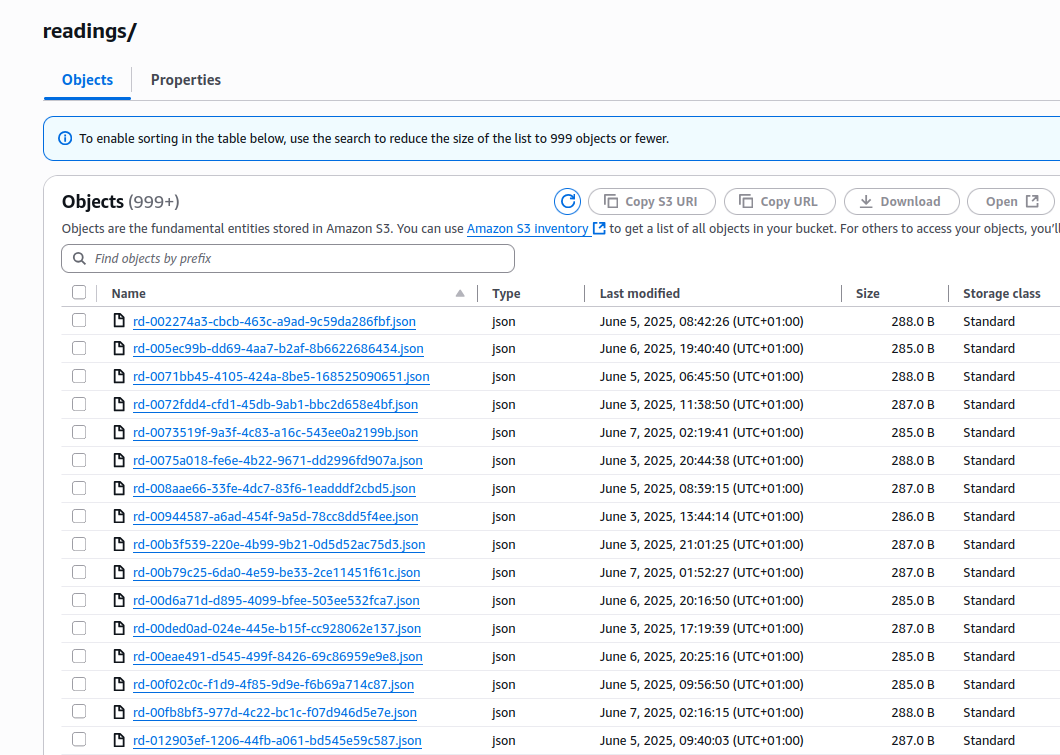
\includegraphics[scale=0.4]{AWS/events_s3_readings}
   \captionof{figure}{Almacenamiento de mensajes JSON en AWS S3.}
   \label{fig:events_s3_readings}
\end{center}


\begin{center}
   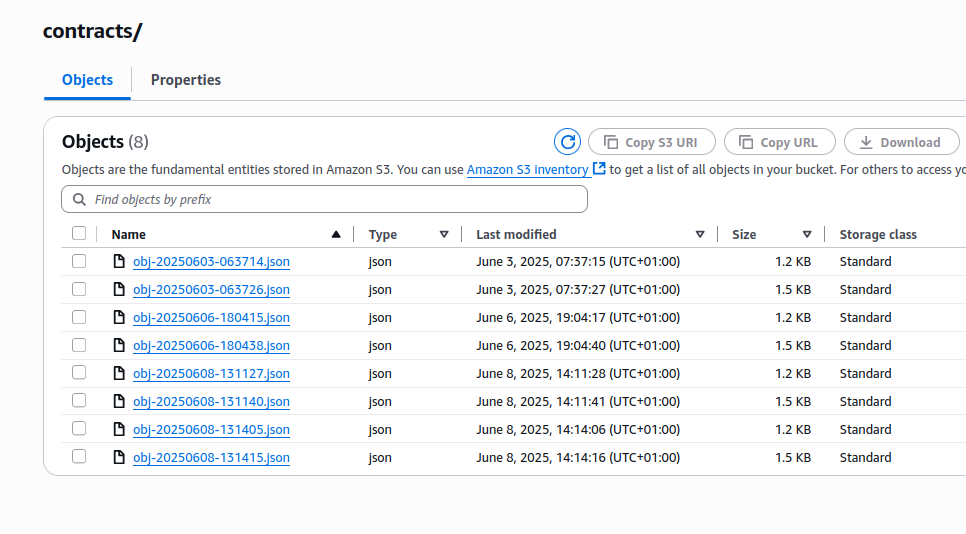
\includegraphics[scale=0.4]{AWS/events_s3_contracts}
   \captionof{figure}{Almacenamiento de mensajes JSON en AWS S3.}
   \label{fig:events_s3_contracts}
\end{center}


\subsection{Verificación del acceso a datos desde AWS Athena}



\begin{center}
   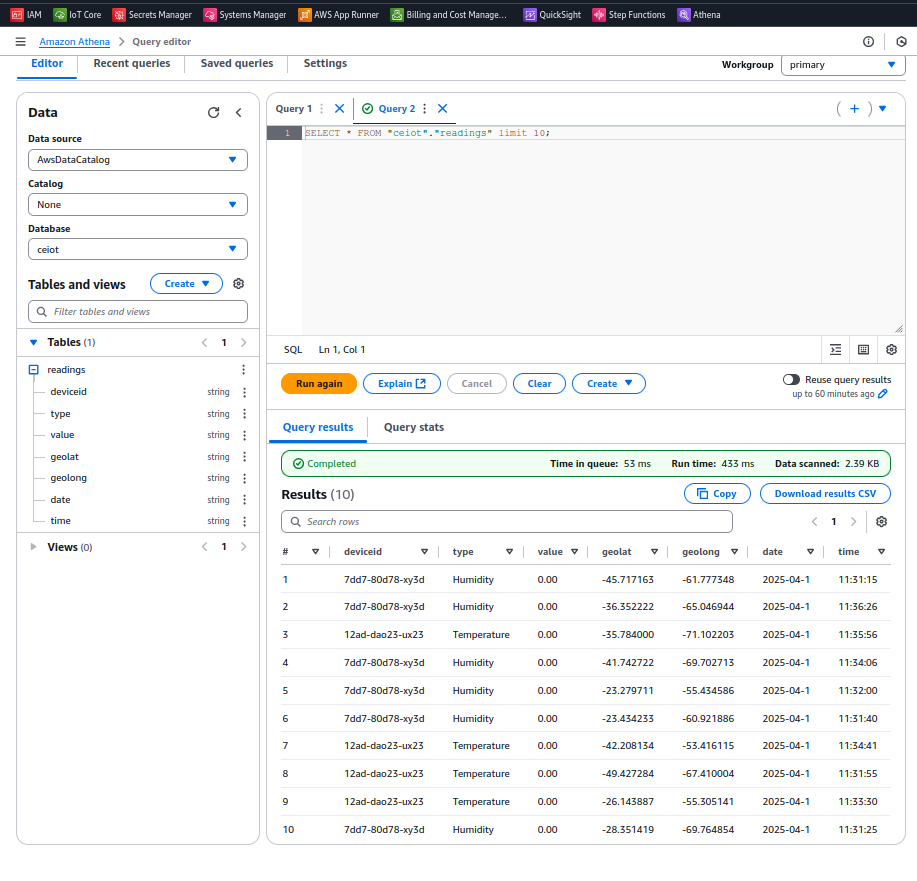
\includegraphics[scale=0.4]{AWS/aws_athena_config}
   \captionof{figure}{Consulta de datos SQL desde AWS Athena.}
   \label{fig:aws_athena_config}
\end{center}





\subsection{Verificación del proceso de ingesta y transformación de datos batch en Fabric}


\begin{center}
   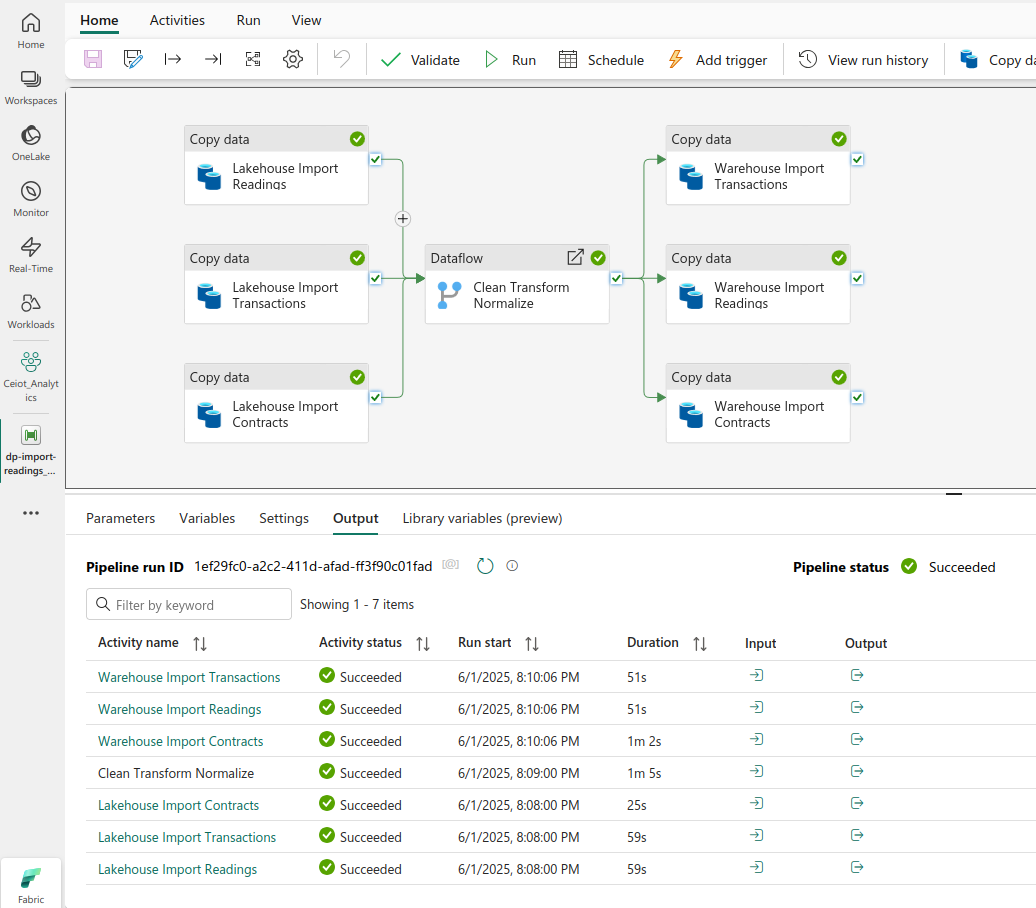
\includegraphics[scale=0.35]{Azure/datafactory_result}
   \captionof{figure}{Correcta ejecución del pipeline punta-a-punta con Azure Data Factory y Dataflows.}
   \label{fig:powerbi1}
\end{center}
 
 

\section{Validaciones funcionales del sistema}



\subsection{Validación del modelo de datos en el Semantic Model}

\subsection{Validación del reporte final generado en PowerBI}


\begin{center}
   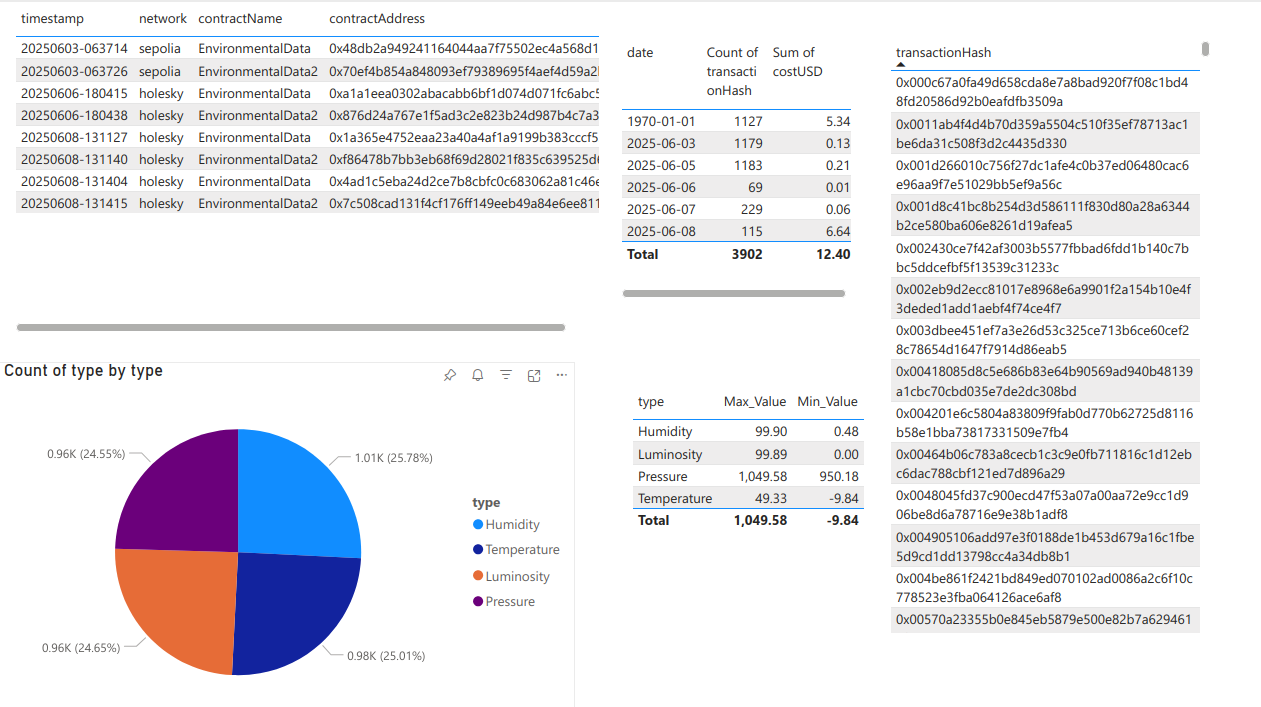
\includegraphics[scale=0.3]{Azure/powerbi_6}
   \captionof{figure}{Dashboard PowerBI.}
   \label{fig:powerbi1}
\end{center}
 
 

\begin{center}
   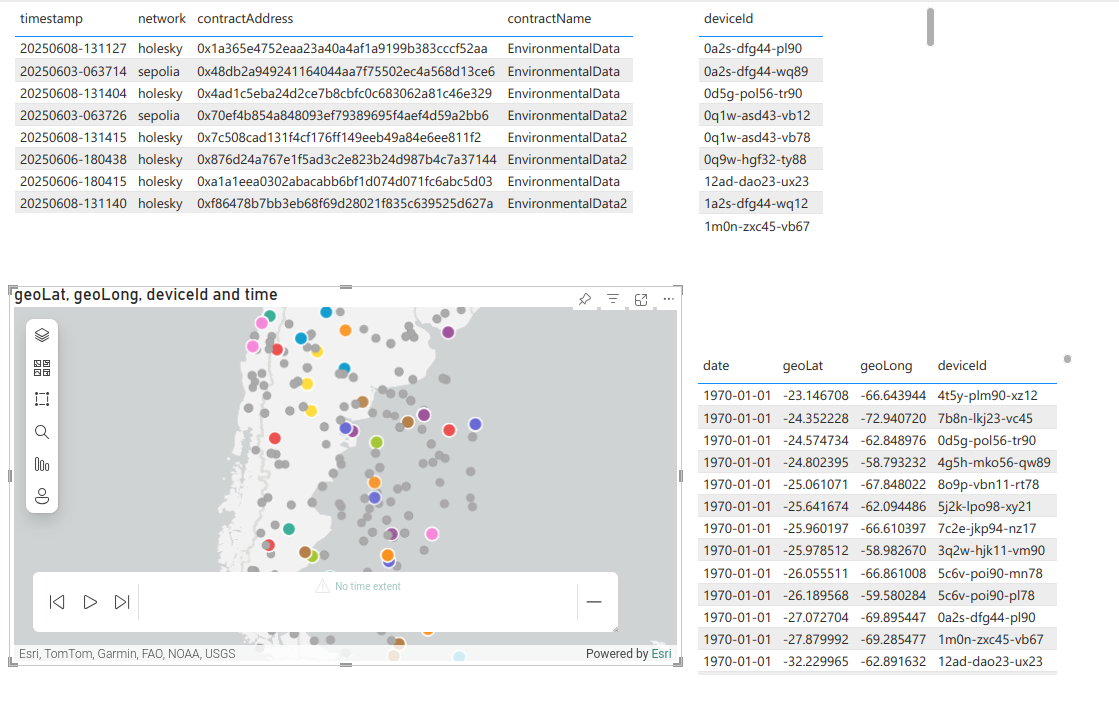
\includegraphics[scale=0.3]{Azure/powerbi_5}
   \captionof{figure}{Dashboard PowerBI.}
   \label{fig:powerbi1}
\end{center}
 


\begin{center}
   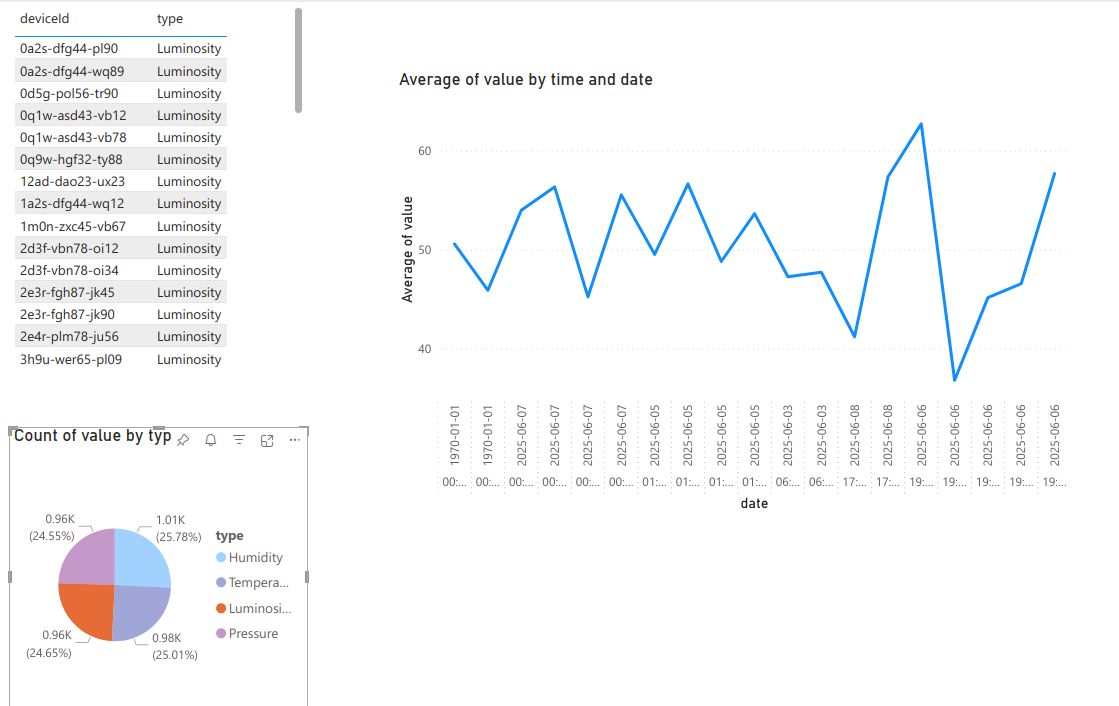
\includegraphics[scale=0.3]{Azure/powerbi_4}
   \captionof{figure}{Dashboard PowerBI.}
   \label{fig:powerbi1}
\end{center}
 
 

\begin{center}
   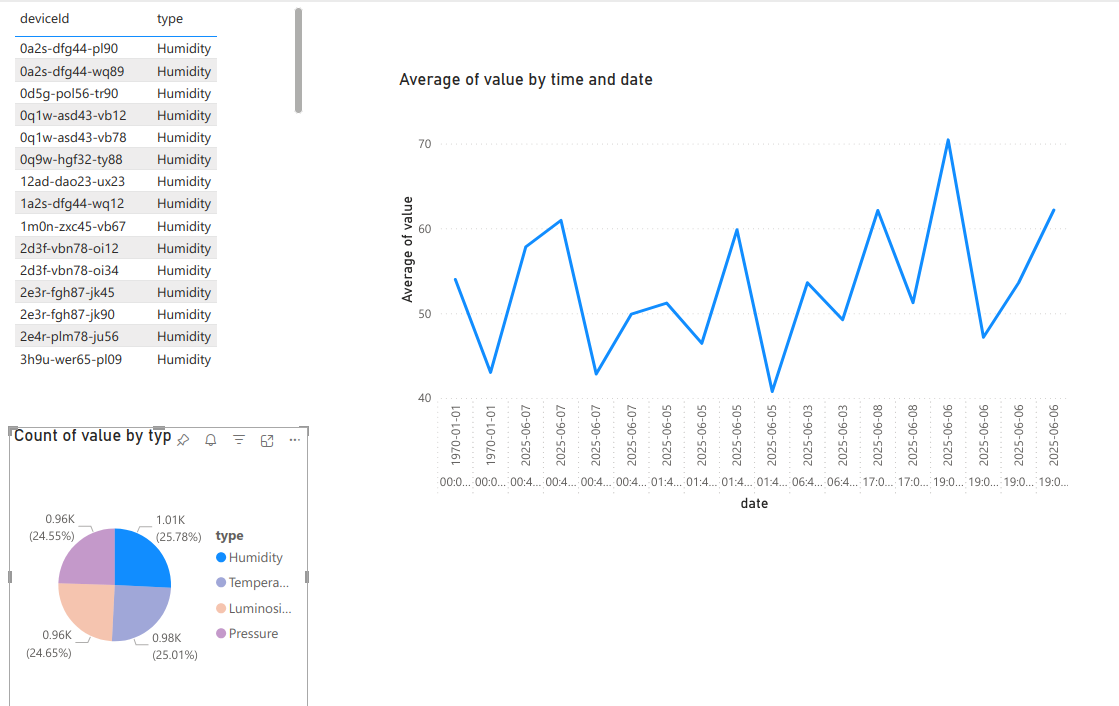
\includegraphics[scale=0.3]{Azure/powerbi_3}
   \captionof{figure}{Dashboard PowerBI.}
   \label{fig:powerbi1}
\end{center}
 
 

\begin{center}
   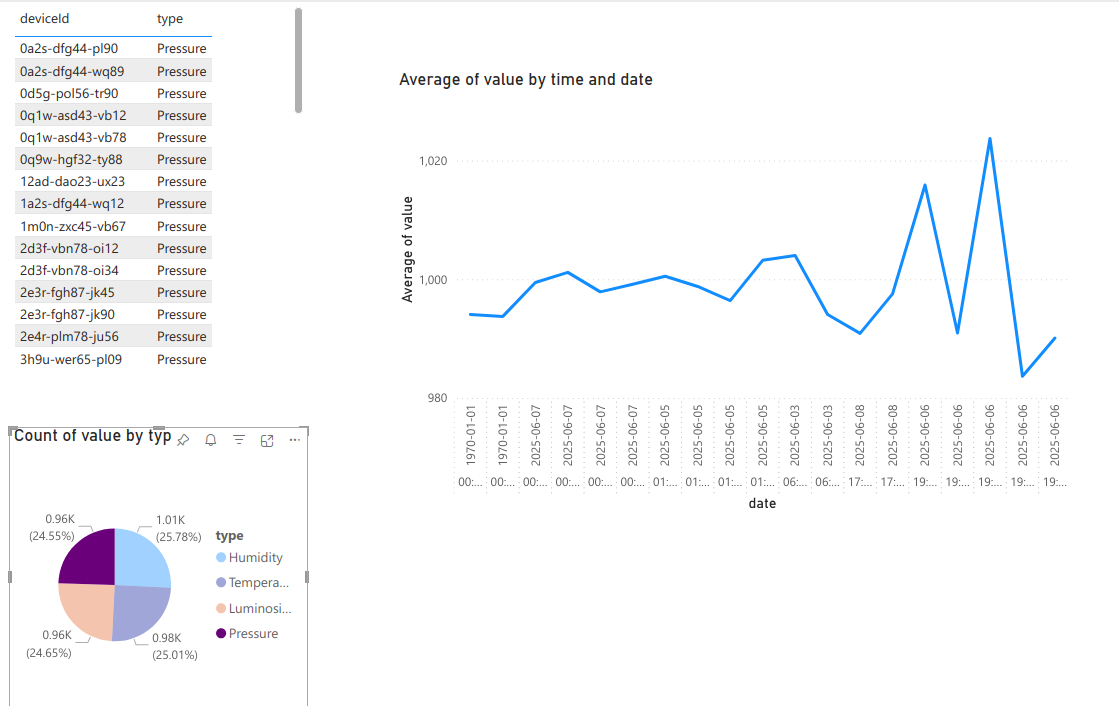
\includegraphics[scale=0.3]{Azure/powerbi_2}
   \captionof{figure}{Dashboard PowerBI.}
   \label{fig:powerbi1}
\end{center}
 
 

\include{Chapters/Chapter5}

%----------------------------------------------------------------------------------------
% Apéndices
%----------------------------------------------------------------------------------------

\appendix

% Incluir apéndices desde archivos separados si es necesario
%\include{Appendices/AppendixA}

%----------------------------------------------------------------------------------------
% Bibliografía
%----------------------------------------------------------------------------------------

\renewcommand{\bibname}{Bibliografía} % Para asegurarte de que el título sea correcto
\phantomsection % Necesario para que el enlace del marcador sea correcto

\printbibliography[heading=bibintoc]

\end{document}






